\documentclass[ngerman,a4paper,order=firstname,sectionreset]{../../texmf/tex/latex/mathscript/mathscript}
\usepackage{../../texmf/tex/latex/mathoperators/mathoperators}

\title{\textbf{Einführung in die Numerik WS2018/19}}
\author{Dozent: Prof. Dr. Andreas Fischer}

\begin{document}
\pagenumbering{roman}
\pagestyle{plain}

\maketitle

\hypertarget{tocpage}{}
\tableofcontents
\bookmark[dest=tocpage,level=1]{Inhaltsverzeichnis}

\pagebreak
\pagenumbering{arabic}
\pagestyle{fancy}

\chapter*{Vorwort}
Schön, dass du unser Skript für die Vorlesung \textit{Lineare Algebra und analytische Geometrie 1} bei Prof. Dr. Arno Fehm im WS2017/18 gefunden hast! \footnote{Obwohl man sagen kann, dass es in dieser Vorlesung nur um Lineare Algebra ging, der Teil mit der analytischen Geometrie wurde vernachlässigt. Liegt wahrscheinlich auch daran, dass es demnächst eine Reform der Studienordnung gibt, in der aus der Vorlesung \textit{Lineare Algebra und analytische Geometrie} die Vorlesung \textit{Einführung in die Lineare Algebra} wird.}

Wir verwalten dieses Skript mittels Github \footnote{Github ist eine Seite, mit der man Quelltext online verwalten kann. Dies ist dahingehend ganz nützlich, dass man die Quelltext-Dateien relativ einfach miteinander synchronisieren kann, wenn man mit mehren Leuten an einem Projekt arbeitet.}, d.h. du findest den gesamten \LaTeX-Quelltext auf \url{https://github.com/henrydatei/TUD_MATH_BA}. Unser Ziel ist, für alle Pflichtveranstaltungen von \textit{Mathematik-Bachelor} ein gut lesbares Skript anzubieten. Für die Programme, die in den Übungen zur Vorlesung \textit{Programmieren für Mathematiker} geschrieben werden sollen, habe ich ein eigenes Repository eingerichtet; es findet sich bei \url{https://github.com/henrydatei/TU_PROG}.

Du kannst dir gerne dort die \LaTeX-Quelldateien herunterladen, die Dateien für exakt dieses Skript sind im Ordner \texttt{1. Semester/LAAG ueberarbeitet}. Es lohnt sich auf jeden Fall während des Studiums die Skriptsprache \LaTeX{} zu lernen, denn Dokumente, die viele mathematische oder physikalische Formeln enthalten, lassen sich sehr gut mittels \LaTeX{} darstellen, in Word oder anderen Office-Programmen sieht so etwas dann eher dürftig aus.

\LaTeX{} zu lernen ist gar nicht so schwierig, ich habe dafür am Anfang des ersten Semesters wenige Wochen benötigt, dann kannte ich die wichtigsten Befehle und konnte den Vorgänger dieses Skriptes schreiben (\texttt{1. Semester/LAAG}, Vorsicht: hässlich, aber der Quelltext ist relativ gut verständlich).

Es sei an dieser Stelle darauf hingewiesen (wie in jedem anderem Skript auch \smiley{}), dass dieses Skript nicht den Besuch der Vorlesungen ersetzen kann. Es könnte sein, dass Prof. Fehm seine Vorlesung immer mal wieder an die Studenten anpasst; wahrscheinlich immer dann, wenn die Prüfungsergebnisse zu schlecht waren. Nichtsdestotrotz veröffentlicht Prof. Fehm sein Skript auf seiner Homepage \url{http://www.math.tu-dresden.de/~afehm/lehre.html}. Allerdings ist dieses Skript recht hässlich, besonders was die Übersichtlichkeit angeht.

Wir möchten deswegen ein Skript bereitstellen, dass zum einen übersichtlich ist, zum anderen \textit{alle} Inhalt aus der Vorlesung enthält, das sind insbesondere Diagramme, die sich nicht im offiziellen Skript befinden, aber das Verständnis des Inhalts deutlich erleichtern. Ich denke, dass uns dies erfolgreich gelungen ist.

Trotz intensivem Korrekturlesen können sich immer noch Fehler in diesem Skript befinden. Es wäre deswegen ganz toll von dir, wenn du auf unserer Github-Seite \url{https://github.com/henrydatei/TUD_MATH_BA} ein neues Issue erstellst und damit auch anderen hilfst, dass dieses Skript immer besser wird.

\chapter{Interpolation}
\section{Grundlagen}

\textbf{Aufgabe:} \\
Gegeben sind $n+1$ Datenpaare $(x_0,f_0),\dots, (x_n,f_n)$, alles reelle Zahlen und paarweise verschieden. \\
Gesucht ist eine Funktion $F:\real\to\real$, die die \begriff{Interpolationsbedingungen}
\begin{align}
	\label{interpolationsbedingung}
	F(x_0) = f_0, \, \dots, \, F(x_n)=f_n
\end{align}
genügt.

\begin{*definition}[Stützstellen, Stützwerte]
	Die $x_0$ bis $x_n$ werden \begriff{Stützstellen} genannt.
	
	Die $f_0$ bis $f_n$ werden \begriff{Stützwerte} genannt.
\end{*definition}

Die oben gestellte Aufgabe wird zum Beispiel durch 
\begin{align}
	F(x) = \begin{cases}
		0 & x\notin \{x_0,\dots,x_n\} \\
		f_i & x=x_i
	\end{cases}\notag
\end{align}
gelöst. Weitere Möglichkeiten sind: Polygonzug, Treppenfunktion, Polynom, \dots
\begin{itemize}
	\item In welcher Menge von Funktionen soll $F$ liegen?
	\item Gibt es im gewählten \begriff{Funktionenraum} für beliebige Datenpaare eine Funktion $F$, die den Interpolationsbedingungen genügt (eine solche Funktion heißt \begriff{Interpolierende})?
	\item Ist die Interpolierende in diesem Raum eindeutig bestimmt?
	\item Welche weiteren Eigenschaften besitzt die Interpolierende, zum Beispiel hinsichtlich ihrer Krümmung oder der Approximation einer Funktion $f:\real\to\real$ mit $f_k=f(x_k)$ für $k=0, \dots, n$
	\item Wie sollte man die Stützstellen wählen, falls nicht vorgegeben?
	\item Wie lässt sich die Interpolierende effizient bestimmen, gegebenenfalls auch unter der Berücksichtigung, dass neue Datenpaare hinzukommen oder dass sich nur die Stützwerte ändern? 
\end{itemize}

\begin{example}
	\hspace*{1.5em}
	\begin{center}
		\begin{tabular}{c|cccccc}
			$k$ & 0 & 1 & 2 & 3 & 4 & 5 \\
			\hline
			$x_k$ in s & 0 & 1 & 2 & 3 & 4 & 5 \\
			\hline
			$f_k$ in °C & 80 & 85,8 & 86,4 & 93,6 & 98,3 & 99,1
		\end{tabular}
	\end{center}
Interpolation im
\begin{itemize}
	\item Raum der stetigen stückweise affinen Funktionen
	\item Raum der Polynome höchstens 5. Grades
	\item Raum der Polynome höchstens 4. Grades (Interpolation im Allgemeinen nicht lösbar, Regression nötig)
\end{itemize}
\end{example}

\section{Interpolation durch Polynome}

$\Pi_n$ bezeichne den Vektorraum der Polynome von Höchstgrad $n$ mit der üblichen Addition und Skalarmultiplikation. Für jedes $p\in\Pi_n$ gibt es $a_0,\dots,a_n\in\real$, sodass
\begin{align}
	p(x) = a_nx^n+a_{n-1}x^{n-1}+\dots+a_1x+a_0
\end{align}
und umgekehrt.

\subsection{Existenz und Eindeutigkeit}

\begin{proposition}
	Zu $n+1$ Datenpaaren $(x_0,f_0),\dots,(x_n,f_n)$ mit paarweise verschiedenen Stützstellen existiert genau ein Polynom $p\in\Pi_n$, dass die Interpolationsbedingung  \cref{interpolationsbedingung} erfüllt.
\end{proposition}
\begin{proof}
	\begin{itemize}
		\item Existenz: Sei $j\in\{0,\dots,n\}$ und $L_j:\real\to\real$ mit
		\begin{align}
			L_j(x) := \prod_{\substack{i=0\\ i\neq j}}^{n} \frac{x-x_i}{x_j-x_i}= \frac{(x-x_0)\cdot\dots\cdot(x-x_{j-1})(x-x_{j+1})\cdot\dots\cdot(x-x_n)} {(x_j-x_0)\cdot\dots\cdot(x_j-x_{j-1})(x_j-x_{j+1})\cdot\dots\cdot(x_j-x_n)}\notag
		\end{align}
		das \begriff{\person{Lagrange}-Basispolynom} vom Grad $n$. Offenbar gilt $L_j\in\Pi_n$ und 
		\begin{align}
			\label{1.3}
			L_j(x_k)=\begin{cases}
				1 & k=j \\ 0 & k\neq j
			\end{cases} = \delta_{jk}
		\end{align}
		Definiert man $p:\real\to\real$ durch
		\begin{align}
			\label{1.4}
			p(x) := \sum_{j=0}^{n} f_j\cdot L_j(x)
		\end{align}
		so ist $p\in\Pi_n$ und außerdem erfüllt $p$ wegen \cref{1.3} die Interpolationsbedingung \cref{interpolationsbedingung}
		\item Eindeutigkeit: Angenommen es gibt Interpolierende $p,\tilde{p}\in\Pi_n$ mit $p\neq\tilde{p}$. Dann folgt $p-\tilde{p}\in\Pi_n$ und $(p-\tilde{p})(x_k)=p(x_k)-\tilde{p}(x_k)=0$ für $k=0,\dots,n$. Also hat $(p-\tilde{p})$ mindestens $n+1$ Nullstellen, hat aber Grad $n$. Das heißt, dass $(p-\tilde{p})$ das Nullpolynom sein muss.
	\end{itemize}
\end{proof}

\begin{*definition}[Interpolationspolynom]
	Das Polynom, dass die Interpolationsbedingung erfüllt, heißt \begriff{Interpolationspolynom} zu $(x_0,f_0),\dots,(x_n,f_n)$.
\end{*definition}

\begin{remark}
	\begin{itemize}
		\item Die Darstellung \cref{1.4} heißt \begriff{\person{Lagrange}-Form} des Interpolationspolynoms.
		\item Um mittels \cref{1.4} einen Funktionswert $p(x)$ zu berechnen, werden $\mathcal{O}(n^2)$ Operationen genötigt; bei gleichabständigen Stützstellen kann man diesen Aufwand auf $\mathcal{O}(n)$ verringern. Ändern sich die Stützwerte, kann man durch Wiederverwendung von den $L_j(x)$ das $p(x)$ in $\mathcal{O}(n)$ Operationen berechnen.
		\item Man kann zeigen, dass $L_0$ bis $L_n$ eine Basis von $\Pi_n$ bilden.
	\end{itemize}
\end{remark}

\section{Interpolation durch Polynomsplines}

\subsection{Polynomsplines}

Zur Abkürzung bezeichne $\Delta$ eine Zerlegung des Intervall $[a,b]$ durch die Stützstellen $a=:x_0<...<x_n:=b$.

\begin{definition}[Polynomspline]
	Ein \begriff{Polynomspline} vom Grad $m\in\natur$ und Glattheit $l\in\natur$ zur Zerlegung $\Delta$ ist eine Funktion $s\in C^l[a,b]$ mit
	\begin{align}
		s_k := s\vert_{[x_k,x_{k+1}]}\in\Pi_n\quad\text{für } k=0,...,n-1\notag
	\end{align}
	Dabei bezeichnet $s\vert_{[x_k,x_{k+1}]}$ die Einschränkung von $s$ auf das Intervall $[x_k,x_{k+1}]$. Die Menge aller Splines wird mit $\mathcal{S}^l_m(\Delta)$ bezeichnet.
	
	Folglich ist ein Polynomspline $s\in\mathcal{S}^l_m(\Delta)$ auf jedem der Teilintervall $[x_k,x_{k+1}]$ ein Polynom vom Höchstgrad $m$. Außerdem ist $s\in\mathcal{S}^l_m(\Delta)$ in allen Punkten $x\in[a,b]$ (also auch in den Stützstellen) $l$-mal stetig differenzierbar. $\mathcal{S}^l_m(\Delta)$ ist mit der üblichen Addition und Multiplikation ein Vektorraum. Speziell ist $\mathcal{S}^0_1(\Delta)$ die Menge aller stetigen stückweise affin linearen Funktionen.
\end{definition}

\begin{center}
	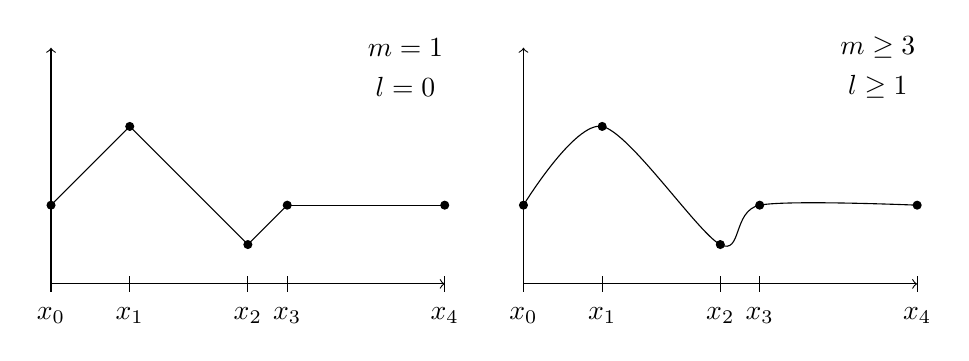
\begin{tikzpicture}
		\draw[->] (0,0) -- (5,0);
		\draw[->] (0,0) -- (0,3);
		
		\draw (0,0.1) -- (0,-0.1);
		\draw (1,0.1) -- (1,-0.1);
		\draw (2.5,0.1) -- (2.5,-0.1);
		\draw (3,0.1) -- (3,-0.1);
		\draw (5,0.1) -- (5,-0.1);
		\node at (0,-0.4) (a) {$x_0$};
		\node at (1,-0.4) (b) {$x_1$};
		\node at (2.5,-0.4) (c) {$x_2$};
		\node at (3,-0.4) (d) {$x_3$};
		\node at (5,-0.4) (e) {$x_4$};
		
		\draw[fill=black] (0,1) circle (0.05);
		\draw[fill=black] (1,2) circle (0.05);
		\draw[fill=black] (2.5,0.5) circle (0.05);
		\draw[fill=black] (3,1) circle (0.05);
		\draw[fill=black] (5,1) circle (0.05);
		\draw (0,1) -- (1,2);
		\draw (1,2) -- (2.5,0.5);
		\draw (2.5,0.5) -- (3,1);
		\draw (3,1) -- (5,1);
		
		\node at (4.5,3) (l) {$m=1$};
		\node at (4.5,2.5) (l) {$l=0$};
		
		\draw[->] (6,0) -- (11,0);
		\draw[->] (6,0) -- (6,3);
		
		\draw (6,0.1) -- (6,-0.1);
		\draw (7,0.1) -- (7,-0.1);
		\draw (8.5,0.1) -- (8.5,-0.1);
		\draw (9,0.1) -- (9,-0.1);
		\draw (11,0.1) -- (11,-0.1);
		\node at (6,-0.4) (a) {$x_0$};
		\node at (7,-0.4) (b) {$x_1$};
		\node at (8.5,-0.4) (c) {$x_2$};
		\node at (9,-0.4) (d) {$x_3$};
		\node at (11,-0.4) (e) {$x_4$};
		
		\draw[fill=black] (6,1) circle (0.05);
		\draw[fill=black] (7,2) circle (0.05);
		\draw[fill=black] (8.5,0.5) circle (0.05);
		\draw[fill=black] (9,1) circle (0.05);
		\draw[fill=black] (11,1) circle (0.05);
		\coordinate (X0) at (6,1);
		\coordinate (X1) at (7,2);
		\coordinate (X2) at (8.5,0.5);
		\coordinate (X3) at (9,1);
		\coordinate (X4) at (11,1);
		\draw[smooth] plot coordinates {(X0) (X1) (X2) (X3) (X4)};
		
		\node at (10.5,3) (l) {$m\ge 3$};
		\node at (10.5,2.5) (l) {$l\ge 1$};
	\end{tikzpicture}
\end{center}

\subsection{Interpolation durch kubische Polynomsplines}

Gegeben sei eine Zerlegung $\Delta$ und die Stützwerte $f_0,...,f_n$. Gesucht ist eine Funktion $s\in\mathcal{S}^l_3(\Delta)$ mit $l=1,2$ derart, dass
\begin{align}
	\label{1.6}
	s(x_k)=f_k\quad\text{für } k=0,...,n
\end{align}
Jede derartige Funktion heißt \begriff{kubischer Interpolationspline}.

\textbf{Konstruktion eines solchen Splines:}
\begin{align}
	h_k &:= x_{k-1}-x_k\quad\text{für } k=0,...,n-1 \notag \\
	m_k &:= s'(x_k) \quad\text{für } k=0,...,n-1\notag
\end{align}
Wegen $l\in\{1,2\}$ ist $s$ zunächst stetig differenzierbar. Wegen $s_k=s\vert_{[x_k,x_{k+1}]}$ für $k=0,...,n-1$ und $m=3$ kann man folgenden Ansatz für $s_k$ benutzen:
\begin{align}
	\label{1.7}
	s_k(x)=a_k(x-x_k)^3+b_k(x-x_k)^2+c_k(x-x_k)+d_k
\end{align}
Aus den Interpolationsbedingungen \cref{1.6} und der stetigen Differenzierbarkeit aller Funktionen in $s\in\mathcal{S}^l_m(\Delta)$ für $l\ge 1$ ergeben sich folgende Forderungen an $s_k$, $k=0,...,n-1$:
\begin{equation}
	\label{1.8}
	\begin{split}
		s_k(x_k) &= f_k \quad\text{und }\quad s_k(x_{k+1}) = f_{k+1} \\
		s'_k(x_k) &= m_k \quad\text{und }\quad s'_k(x_{k+1}) = m_{k+1}
	\end{split}
\end{equation}
Diese liefern:
\begin{equation}
	\label{1.9}
	\begin{split}
		d_k &= s_k(x_k)=f_k \\
		c_k &= s'_k(x_k)=m_k
	\end{split}
\end{equation}
und damit:
\begin{align}
	s_k(x_{k+1}) &= a_kh_k^3 + b_kh_k^2+m_kh_k + f_k = f_{k+1} \notag \\
	s'_k(x_{k+1}) &= 3a_kh_k^2 + 2b_kh_k + m_k = m_{k+1} \notag
\end{align}
Damit ergeben sich $a_k$ und $b_k$ als eindeutige Lösung für das lineare Gleichungssystem
\begin{align}
	\label{1.10}
	\begin{pmatrix}
		h_k^3 & h_k^2 \\ 3h_k^2 & 2h_k
	\end{pmatrix}
	\begin{pmatrix}
		a_k \\ b_k
	\end{pmatrix}=
	\begin{pmatrix}
		f_{k+1}-f_k-m_kf_k \\
		m_{k+1}-m_k
	\end{pmatrix}
\end{align}
Die Determinante ist $-h_k^4\neq 0$.

\begin{proposition}
	Sei eine Zerlegung $\Delta$ des Intervalls $[a,b]$ gegeben. Dann gibt es für beliebig gewählte reelle Zahlen $f_0,...,f_n$ und $m_0,...,m_n$ einen Interpolationsspline $s\in\mathcal{S}^1_3(\Delta)$, der den Interpolationsbedingungen
	\begin{align}
		s'(x_0)=m_0,...,s'(x_n)=m_n\notag
	\end{align}
	genügt. Außerdem gilt: $s\vert_{[x_k,x_{k+1}]}=s_k$ für k=0,...,n-1 mit $s_k$ entsprechend \cref{1.7}, wobei sich $a_k,b_k,c_k,d_k$ aus \cref{1.9} und \cref{1.10} ergeben.
\end{proposition}

Für die Wahl der $m_k$ gibt es verschiedene Möglichkeiten, zum Beispiel:
\begin{itemize}
	\item Falls Ableitungswerte der zu interpolierenden Funktion $f$ bekannt sind, kann man $m_k=f'(x_k)$ setzen.
	\item Man wählt $m_0,...,m_n$ so, dass $s$ zweimal stetig differenzierbar ist, das heißt $s\in\mathcal{S}^2_3(\Delta)$ statt  $s\in\mathcal{S}^1_3(\Delta)$ gilt.
\end{itemize}

\subsection{Interpolation mit kubischen $C^2$-Splines}

Damit ein kubischer Interpolationsspline $s$ zu $\mathcal{S}^2_3(\Delta)$ gehört, muss neben den Forderungen in \cref{1.8} die Stetigkeit von $s''$ an den Stützstellen $x_1,...,x_{n-1}$ gewährleistet sein. Also hat man zusätzliche Bedingungen
\begin{align}
	s''_k(x_{k+1})=s''_{k+1}(x_{k+1})\quad\text{für } k=0,...,n-2\notag
\end{align}
\begin{center}
	\begin{tikzpicture}
		\draw[bend left] (0,0) to (2,1);
		\draw[out=0] (2,1) to [in=180] (4,2);
		\draw[out=0] (4,2) to [in=120] (6,0);
		
		\node at (1,2.5) (s1) {$s_k$};
		\node at (3,2.5) (s2) {$s_{k+1}$};
		\node at (5,2.5) (s3) {$s_{k+2}$};
		
		\draw[dashed] (2,0) -- (2,2.7);
		\draw[dashed] (4,0) -- (4,2.7);
		\node at (2,-0.3) (a) {$x_{k+1}$};
		\node at (4,-0.3) (b) {$x_{k+2}$};
		
		\draw[->] (1.5,0) -- (1.9,0);
		\draw[->] (2.5,0) -- (2.1,0);
		\draw[->] (3.5,0) -- (3.9,0);
		\draw[->] (4.5,0) -- (4.1,0);
	\end{tikzpicture}
\end{center}
Mit \cref{1.7} ergibt sich $s''(x)=6a_k(x-x_0)+2b_k$ für $x\in[x_k,x_{k+1}]$ und damit $s''_k(x_{k+1}) = 6a_kh_k+2b_k$ und $s''_{k+1}(x_{k+1})=2b_{k+1}$, also 
\begin{align}
	\label{1.11}
	3a_kh_k+b_k=b_{k+1}\quad\text{für }k=0,...,n-2
\end{align}
Aus \cref{1.10} folgt
\begin{align}
	a_k &= \frac{-2}{h_k^3}(f_{k+1}-f_k)+\frac{1}{h_k^2}(m_k+m_{k+1}) \notag \\
	b_k &= \frac{3}{h_k^2}(f_{k+1}-f_k)-\frac{1}{h_k}(2m_k+m_{k+1})\notag
\end{align}
für $k=0,...,n-1$. Wegen \cref{1.11} erhält man für $k=0,...,n-2$
\begin{align}
	& \frac{-6}{h_k^2}(f_{k+1}-f_k) + \frac{3}{h_k}(m_k+m_{k+1}) + \frac{3}{h_k^2}(f_{k+1}-f_k) - \frac{1}{h_k}(2m_k+m_{k+1}) \notag \\
	&= \frac{-6}{h^2_{k+1}}(f_{k+2}-f_{k+1})-\frac{1}{h_{k+1}}(2m_{k+1}+m_{k+2})\notag
\end{align}
Damit folgt 
\begin{align}
	\frac{1}{h_k}(m_k+2m_{k+1}) + \frac{1}{h_{k+1}}(2m_{k+1}+m_{k+2}) &= \frac{3}{h_k^2}(f_{k+1}-f_k) + \frac{3}{h_{k+1}^2}(f_{k+2}-f_{k+1})\notag \\
	\text{bzw.}\quad h_{k+1}m_k + 2(h_{k+1}+h_k)m_{k+1}+h_km_{k+2} &= \frac{3h_{k+1}}{h_k}(f_{k+1}-f_k) + \frac{3h_k}{h_{k+1}}(f_{k+2}-f_{k+1})\notag
\end{align}
Also müssen die $n+1$ Zahlen $m_0,...,m_n$ den $n-1$ Gleichungen des linearen Gleichungssystems 
\begin{align}
	\begin{pmatrix}
		\lambda_0 & 2 & \mu_0 & & & \\
		 & \lambda_1 & 2 & \mu_1 & & \\
		 & & \ddots & \ddots & \ddots & \\
		 & & & \lambda_{n-2} & 2 & \mu_{n-2}
	\end{pmatrix}
	\begin{pmatrix}
		m_0 \\ m_1 \\ \vdots \\ m_n
	\end{pmatrix}
	= \begin{pmatrix}
	 r_0 \\ r_1 \\ \vdots \\ r_{n-2}
	\end{pmatrix}\notag
\end{align}
genügen, wobei $\lambda_k,\mu_k,r_k$ durch
\begin{align}
	\lambda_k &= \frac{h_{k+1}}{h_k+h_{k+1}} \notag \\
	\mu_k &= \frac{h_k}{h_k + h_{k+1}}\notag \\
	r_k &= \frac{3h_{k+1}}{h_k(h_k+h_{k+1})}(f_{k+1}-f_k) + \frac{3h_k}{h_{k+1}(h_k+h_{k+1})}(f_{k+2} - f_{k+1})\notag
\end{align}
für $k=0,...,n-2$ gegeben sind. Die Systemmatrix und die erweiterte Systemmatrix haben den Rang $n-1$. Somit ist das Gleichungssystem lösbar, besitzt aber keine eindeutige Lösung. Um solche zu erhalten, kann man zusätzliche Bedingungen stellen, etwa
\begin{enumerate}[label=(\alph*)]
	\item \textbf{natürliche Randbedingungen:} 
	\begin{align}
		\label{1.12}
		s''(x_0) = s''(x_n)=0
	\end{align}
	Diese sind gleichbedeutend mit 
	\begin{align}
		s''_0(x_0)=6a_0(x-x_0)+2b_0=0\quad\text{und}\quad s''_{n-1}(x_n)=6a_{n-1}(x_n-x_{n-1})+2b_{n-1}=0\notag
	\end{align}
	Also folgt
	\begin{align}
		b_0=0\quad\text{und}\quad 3a_{n-1}h_{n-1} + b_{n-1}=0\notag
	\end{align}
	Nutzt man noch die Darstellung für $b_0$ sowie für $a_{n-1}$ und $b_{n-1}$, so folgt
	\begin{align}
		2m_0+m_1 = \frac{3}{h_0}(f_1-f_0) \quad\text{und}\quad m_{n-1}+2m_n=\frac{3}{h_{n-1}}(f_n-f_{n-1})\notag
	\end{align}
	Fügt man beide Gleichungen geeignet zum obigen System hinzu, erhält man ein lineares Gleichungssystem mit einer regulären trigonales Systemmatrix. Dieses kann in $\mathcal{O}(n)$ Operationen gelöst werden.
	\item \textbf{Vollständige Randbedingungen:} Sind $f'(a)$ und $f'(b)$ bekannt, dann können die zusätzlichen Bedingungen
	\begin{align}
		\label{1.13}
		s'(x_0)=f'(a)\quad\text{und}\quad s'(x_n)=f'(b)
	\end{align}
	mittels $m_0=f'(a)$ und $m_n=f'(b)$ geeignet in das Gleichungssystem eingefügt werden, so dass man analog zu Fall (a) eine trigonale reguläre Systemmatrix erhält.
	\item \textbf{Periodische Spline-Interpolation:} Falls
	\begin{align}
		\label{1.14}
		f'(a)=f'(b)
	\end{align}
	und $f''(a)=f''(b)$ gilt, dann sind 
	\begin{align}
	\label{1.15}
		s'(x_0)=s'(x_n)\quad\text{und}\quad s''(x_0)=s''(x_n)
	\end{align}
	sinnvolle Randbedingungen, woraus sich zwei zusätzliche lineare Gleichungen zur Ergänzung des Gleichungssystems ableiten lassen.
	\item (nicht in der Vorlesung) \textbf{Not-in-knot Bedingung:} Es soll zusätzlich
	\begin{align}
		s'''_0(x_1)=s'''_1(x_1) \quad\text{und}\quad s'''_{n-2}(x_{n-1})=s'''_{n-1}(x_{n-1})\notag
	\end{align}
	gelten, das heißt $s$ ist auf $[x_0,x_2]$ und auf $[x_{n-2},x_n]$ ein Polynom dritten Grades. Man erhält daraus die Forderungen $a_0=a_1$ und $a_{n-2}=a_{n-1}$, woraus sich zusätzliche Gleichungen in den Variablen $m_0,m_1,m_2$ und $m_{n-2},m_{n-1},m_n$ ergeben.
\end{enumerate}

\subsection{Eine Minimaleigenschaft kubischer $C^2$-Interpolationssplines}

Durch
\begin{align}
	\skalar{f}{g}:= \int_a^b f(x)g(x)\diff x\quad\text{bzw.}\quad\Vert g\Vert_2:=\sqrt{\int_a^b g(x)^2\diff x} \quad\text{ für } f,g\in L^2[a,b]\notag
\end{align}
ist ein Skalarprodukt bzw. eine Norm in $L^2[a,b]$ definiert.

\begin{proposition}
	\proplbl{satz_1_6}
	Seien $f\in C^2[a,b]$, $\Delta$ eine Zerlegung von $[a,b]$ und $f_k:=f(x_k)$ für $k=0,...,n$. Für einen Interpolationsspline $s\in\mathcal{S}^2_3(\Delta)$, der die natürlichen, vollständigen oder periodischen Randbedingungen (bei letzteren gelte \cref{1.14}) erfüllt, gilt:
	\begin{align}
		\Vert s''\Vert^2_2 = \Vert f''\Vert_2^2 - \Vert f''-s''\Vert_2^2 \le \Vert f''\Vert_2^2\notag
	\end{align}
\end{proposition}
\begin{proof}
	Durch Nachrechnen sieht man
	\begin{align}
		\int_a^b (f''(x))^2\diff x-\int_a^b (f''(x)-s''(x))^2\diff x = \int_a^b (s''(x))^2\diff x + 2\int_a^b \left[ f''(x)-s''(x)\right] s''(x)\diff x \notag
	\end{align}
	Es wird nun $J:=\int_a^b \left[ f''(x)-s''(x)\right] s''(x)\diff x=0$ gezeigt. Mit Hilfe partieller Integration folgt
	\begin{align}
		J=\left[ f'(x)-s'(x)\right] s''(x)\vert_a^b - \int_a^b \left[ f'(x)-s'(x)\right] s'''(x)\diff x\notag
	\end{align}
	wobei $s'''$ auf jedem Teilintervall $[x_k,x_{k+1}]$ konstant ist. Dies ergibt wegen \cref{1.6}
	\begin{align}
		\int_a^b \left[ f'(x)-s'(x)\right] s'''(x)\diff x &= \sum_{k=0}^{n-1} s'''\left(x_k+\frac{h_k}{2}\right)\int_{x_k}^{x_{x+1}}f'(x)-s'(x)\diff x \notag \\
		&= \sum_{k=0}^{n-1} s'''\left(x_k+\frac{h_k}{2}\right)\big(\big[f(x_{k+1})-s(x_{k+1})\big]-\big[f(x_k)-s(x_k)\big]\big) \notag \\
		&= 0 \notag
	\end{align}
	und damit 
	\begin{align}
		J=\left[ f'(x)-s'(x)\right] s''(x)\vert_a^b = \left[ f'(b)-s'(b)\right] s''(b)-\left[ f'(a)-s'(a)\right] s''(a)\notag
	\end{align}
	Nutzt man nun noch \cref{1.12}, \cref{1.13} bzw. \cref{1.14} mit \cref{1.15}, so folgt $J=0$.
\end{proof}

\begin{*anmerkung}
	\begin{itemize}
		\item \cref{1.12}: natürliche Randbedingungen: $s''(a)=s''(b)=0$
		\item \cref{1.13}: vollständige Randbedingungen: $s(a')=f'(a)$, $s'(b)=f'(b)$
		\item \cref{1.14} und \cref{1.15}: periodische Randbedingungen: $s'(a)=s'(b)$, $s''(a)=s'(b)$, $f'(a)=f'(b)$
	\end{itemize}
\end{*anmerkung}

\subsection{Interpolationsfehler bei kubischer $C^2$-Interpolation}

\begin{*anmerkung}
	Die \person{Cauchy-Schwarz}-Ungleichung hat folgende Form:
	\begin{align}
		\vert\skalar{f}{g}\vert \le \Vert f\Vert_2\cdot\Vert g\Vert_2\notag
	\end{align}
\end{*anmerkung}

\begin{proposition}
	Seien $f\in C^2[a,b]$, $\Delta$ eine Zerlegung von $[a,b]$ und $f_k:=f(x_k)$ für $k=0,...,n$. Für einen Interpolationsspline $s\in\mathcal{S}^2_3(\Delta)$, der die natürlichen, vollständigen oder periodischen Randbedingungen (bei letzteren gelte \cref{1.14}) erfüllt, gilt:
	\begin{align}
		\Vert f-s\Vert_\infty \le \frac{1}{2}h^{\sfrac{3}{2}}\Vert f''\Vert_2\notag
	\end{align}
	wobei $h:=\max\{h_0,...,h_{n-1}\}$.
\end{proposition}
\begin{proof}
	Die Funktion $r:=f-s$ hat wegen \cref{1.6} die $n+1$ Nullstellen $x_0,...,x_n$. Der maximale Abstand benachbarter Nullstellen ist $h$. Nach dem Satz von Rolle besitzt $r'$ mindestens $n$ Nullstellen. Der Abstand zweier Nullstellen von $r'$ ist durch $2h$ nach oben beschränkt. Sei $z\in [a,b]$ so gewählt, dass $\vert r'(z)\vert=\Vert r'\Vert_\infty$. Dann gilt $\vert z-z^0\vert\le h$ für die $z$ am nächsten liegende Nullstelle $z^0$ von $r'$. O.B.d.A. sei $z^0\le z$. Mit der \person{Cauchy-Scharz}-Ungleichung folgt:
	\begin{align}
		\label{1.16}
		\begin{split}
		\Vert r'\Vert_\infty^2 &= \vert r'(z)-\underbrace{r'(z^0)}_{z^0\text{ NST}}\vert^2 \\
		&\overset{\ast}{=} \left|\int_{z^0}^z r''(x)\cdot 1\diff x\right|^2  \\
		&\overset{\tiny{\text{CS}}}{\underset{\tiny{\text{UG}}}{\le}} \int_{z^0}^z r''(x)^2\diff x\cdot \underbrace{\int_{z^0}^z 1^2\diff x}_{=z-z^0\le h} \\
		&\le h\Vert r''\Vert_2^2
		\end{split}
	\end{align}
	$\ast$: Anwendung des Hauptsatzes der Integralrechnung
	
	
	Sei nun $y\in[a,b]$ so gewählt, dass $\vert r(y)\vert=\Vert r\Vert_\infty$. Dann gilt $\vert y-y_0\vert\le \sfrac{h}{2}$ für die $y$ am nächsten liegende Nullstelle $y^0$ von $r$. O.B.d.A. sei $y^0\le y$. Mit \cref{1.16} ergibt sich
	\begin{align}
		\Vert r\Vert_\infty = \vert r(y)-r(y^0)\vert=\left|\int_{y^0}^y r'(x)\diff x\right|\le\max\vert r'(x)\vert\cdot \int_{y^0}^y \diff x\le \frac{1}{2}\Vert r'\Vert_\infty\le \frac{1}{2}h^{\sfrac{3}{2}}\Vert r''\Vert_2\notag
	\end{align}
	Mit \propref{satz_1_6} hat man $\Vert r''\Vert_2\le \Vert f\Vert_2$ und damit die Behauptung.
\end{proof}

\begin{remark}
	Besitzt $f$ eine höhere Glattheit, so kann die obige Fehlerschranke bezüglich der $h$-Potenz verbessert werden. Es lassen sich ferner Abschätzungen für $\Vert f'-s'\Vert_\infty$ und $\Vert f''-s''\Vert_\infty$ herleiten.
\end{remark}


\chapter{numerische Integration (Quadratur)}
\section{Integration von Interpolationspolynomen}
\section{\person{Newton-Cotes}-Formeln}

Falls die Stützstellen gleichabständig sind mit $x_0=a$ und $x_n=b$, das heißt
\begin{align}
	\label{2.1}
	x_{k+1}=x_k+h\quad\text{für } k=0,...,n-1
\end{align}
mit der Schrittweite $h=\frac{b-a}{n}$ gilt, so nennt man $Q_n(f)$ \begriff[Newton-Cotes-Formel!]{geschlossene \person{Newton-Cotes}-Formel}. Ist $a<x_0$ und $x_n<b$ und gilt \cref{2.1} mit $h=\frac{b-a}{n+2}$, so bezeichnet man $Q_n(f)$ als \begriff[Newton-Cotes-Formel!]{offene \person{Newton-Cotes}-Formel}. Im Folgenden wollen wir uns auf den Fall geschlossener \person{Newton-Cotes}-Formeln beschränken.
\section{spezielle \person{Newton-Cotes}-Formeln}
\section{Zusammengesetzte \person{Newton-Cotes-Formeln}}
\section{\person{Gauss}'sche Quadraturformeln}

\chapter{direkte Verfahren für lineare Gleichungssysteme}
\section{\person{Gauss}'scher Algorithmus für quadratische Systeme}

\subsection{Grundform des \person{Gauss}'schen Algorithmus}

\begin{example}
	\begin{align}
		\sysdelim{.}{.}\systeme{2x_1-2x_2+4x_3=10@E_{*},x_1+3x_2+6x_3=25,-x_1+2x_2+x_3=6}\notag
	\end{align}
	$E_1$ behalten $\to E_1'$, $E_2-\frac{1}{2}E_1\to E_2'$, $E_3+\frac{1}{2}E_1\to E_3'$
	\begin{align}
		\sysdelim{.}{.}\systeme{2x_1-2x_2+4x_3=10@E'_{*},4x_2+4x_3=20,x_2+3x_3=11}\notag
	\end{align}
	$E_1'$ behalten $\to E_1''$, $E_2'$ behalten $\to E_2''$, $E_3'-\frac{1}{4}E_2'\to E_3''$
	\begin{align}
		\sysdelim{.}{.}\systeme{2x_1-2x_2+4x_3=10@E''_{*},4x_2+4x_3=20,2x_3=6}\notag
	\end{align}
	$\Rightarrow x_3=3$, $x_2=2$, $x_1=1$
\end{example}

Alle drei Systeme sind äquivalent, das heißt ihre Lösungsmengen sind gleich. Das letzte System wird \begriff{Dreieckssystem} oder System in \begriff{Zeilenstufenform} oder \begriff{gestaffeltes System} genannt.

Gegeben seien $A=(a_{ij})\in\real^{n\times n}$ und $b=(b_i)\in\real^n$. Gesucht ist, falls vorhanden, eine Lösung des linearen Gleichungssystems
\begin{align}
	\begin{array}{ccccccc}
		a_{11}x_1 & + & ... & + & a_{1n}x_n & = & b_1 \\
		\vdots & && & \vdots & \vdots & \vdots \\
		a_{n1}x_1 & + & ... & + & a_{nn}x_n & = & b_n
	\end{array}\notag
\end{align}
bzw. in Matrix-Schreibweise: $Ax=b$.

\subsubsection*{Prinzipielles Vorgehen}

\begin{enumerate}[label=\textbf{\arabic*.}]
	\item Vorwärtselimination (unter Voraussetzung der Durchführbarkeit): Schrittweise Transformation der erweiterten Koeffizientenmatrix
	\begin{align}
		(A,b) = (A^{(1)},b^{(1)})\to (A^{(2)},b^{(2)})\to ...\to (A^{(n)},b^{(n)})=(U,z)\notag
	\end{align}
	wobei $U$ eine obere Dreiecksmatrix ist. Der Eliminationsschritt $(A^{(k)},b^{(k)})\to(A^{(k+1)},b^{(k+1)})$ für $k=1,...,n-1$ verwendet die Eliminationsfaktoren
	\begin{align}
		l_{ik} = \frac{a_{ik}^{(k)}}{a_{kk}^{(k)}}\notag
	\end{align}
	um die $i$-te Zeile der neuen Matrix aus der alten Matrix zu bestimmen
	\begin{align}
		\text{neue Zeile }i &= \text{alte Zeile }i &\text{für } i=1,...,k \notag \\
		\text{neue Zeile }i &= \text{alte Zeile }i - l_{ik}\cdot\text{neue Zeile }k &\text{für } i=k+1,...,n\notag
	\end{align}
	\item Rücksubstitution (unter Voraussetzung der Durchführbarkeit): Lösung des Gleichungssystems $Ux=z$ nach $x$ für gegebenes $U,z$
\end{enumerate}

\begin{algorithm}[Vorwärtselimination]
	\proplbl{3_1_2}
	Input: $n$, $A$, $b$
\begin{lstlisting}
do k= 1, n-1
 do i = k+1, n
  %$l_{ik}$% = %$a_{ik}$% / %$a_{kk}$%
  %$b_i$% = %$b_i$% - %$l_{ik}b_k$%
  do j = k+1, n 
   %$a_{ij}$% = %$a_{ij}$% - %$l_{ik}a_{kj}$%
  end do
 end do
end do
\end{lstlisting}
	Output: $(U,z)$ und $l_{ik}$ für $i>k$. $U$ steht in der oberen Hälfte von $A$ mit Hauptdiagonale, $b$ enthält $z$, die Zahlen $l_{ik}$ lassen sich in der unteren Hälfte von $A$ abspeichern.
\end{algorithm}

\begin{algorithm}[Rücksubstitution]
	\proplbl{3_1_3}
	Input: $n$, $U$, $z$
\begin{lstlisting}
do i = n, 1, -1
 s = 0
 do j = i+1, n
  s = s + %$u_{ij}x_j$%
 end do
end do
\end{lstlisting}
	Output: $x$
\end{algorithm}

Der Aufwand bei uneingeschränkter Durchführbarkeit von \propref{3_1_2} ist $\sim \frac{2}{3}n^3$ und \propref{3_1_3} ist $\sim n^2$

\subsubsection*{Durchführbarkeit}

Der \propref{3_1_2} ist genau dann durchführbar, wenn $a_{kk}^{(k)}\neq 0$ für alle $k=1,...,n-1$ gilt. Gilt auch $a_{nn}^{(n)}\neq 0$, so folgt $u_{ii}\neq 0$ für $i=1,...,n$ und damit die Durchführbarkeit von \propref{3_1_3}.

\begin{definition}[streng diagonaldominant]
	Eine Matrix $A=(a_{ij})\in\real^{n\times n}$ heißt \begriff{streng diagonaldominant}, wenn
	\begin{align}
		\vert a_{ii}\vert > \sum_{\substack{j=1\\ j\neq i}}^{n}\vert a_{ij}\vert\quad\text{für alle } i=0,...,n\notag
	\end{align}
\end{definition}

\begin{lemma}
	Ist die Matrix $A\in\real^{n\times n}$ streng diagonaldominant, so sind \propref{3_1_2} und \propref{3_1_3} durchführbar
\end{lemma}
\begin{proof}[nicht in der Vorlesung]
	Die Matrix $A^{(1)}$ sei streng diagonaldominant. Weiter seien die Matrizen $A^{(k)}$ für ein $k\in\{1,...,n-1\}$ durch Vorwärtselimination erzeugt und streng diagonaldominant. Dies zieht $\vert a_{kk}^{(k)}\vert >0$ nach sich, so dass die Erzeugung von $A^{(k+1)}$ durch Vorwärtselimination wohldefiniert ist. Es wird nun gezeigt, dass $A^{(k+1)}$ wieder streng diagonaldominant ist. Da $A^{(1)}=A$ als streng diagonaldominant vorausgesetzt wurde, folgt dann die Durchführbarkeit der gesamten Vorwärtselimination durch vollständige Induktion. Sei $i>k$ eine Zeile der Matrix $A^{(k+1)}$. Dann hat man
	\begin{align*}
		\sum_{\substack{j=1\\ j\neq i}}^n \vert a_{ij}^{(k+1)}\vert \sum_{\substack{j=k+1\\ j\neq i}}\vert a_{ij}^{(k+1)}\vert &= \sum_{\substack{j=k+1\\ j\neq i}}^n \left|a_{ij}^{(k)} - \frac{a_{kj}^{(k)} a_{ik}^{(k)}}{a_{kk}^{(k)}}\right| \\
		&\le \sum_{\substack{j=k+1\\ j\neq i}}^n \vert a_{ij}^{(k)}\vert + \left|\frac{a_{ik}^{(k)}}{a_{kk}^{(k)}}\right| \sum_{\substack{j=k+1\\ j\neq i}}^n \vert a_{kj}^{(k)}\vert \\
		&< \vert a_{ii}^{(k)}\vert - \vert a_{ik}^{(k)}\vert + \left|\frac{a_{ik}^{(k)}}{a_{kk}^{(k)}}\right| \left( \vert a_{kk}^{(k)}\vert - \vert a_{ki}^{(k)}\vert  \right) \\
		&= \vert a_{ii}^{(k)}\vert  - \left|\frac{a_{ik}^{(k)} a_{ki}^{(k)}}{a_{kk}^{(k)}}\right| \\
		&\le \left| a_{ii}^{(k)} - \frac{a_{ik}^{(k)} a_{ki}^{(k)}}{a_{kk}^{(k)}} \right| \\
		&= \vert a_{ii}^{(k+1)}\vert
	\end{align*}
	Falls $i\le k$, so ändert sich $A^{(k+1)}$ gegenüber $A^{(k)}$ bezüglich der Zeile $i$ nicht. Also ist $A^{(k+1)}$ streng diagonaldominant und man schließt auf die Durchführbarkeit der Vorwärtselimination für $k=1,...,n-1$ und insbesondere auf $\vert a_{ii}^{(n)}\vert >0$ für $i=1,...,n$. DIe Matrix $A^{(n)}$ enthält die Matrix $U$ im oberen Dreieck, deren Diagonalelemente sind gerade $a_{11}^{(n)},...,a_{nn}^{(n)}$, also ist auch die Rücksubstitution wohldefiniert.
\end{proof}

\subsection{Pivotisierung}

Die Regularität der Matrix $A\in\real^{n\times n}$ ist zwar äquivalent zur Lösbarkeit des linearen Gleichungssystems $Ax=b$, für jeden beliebigen Vektor $b\in\real^n$, jedoch sichert die Regularität nicht die Durchführbarkeit der Grundform des \person{Gauss}'schen Algorithmus. Um die Durchführbarkeit bei regulärem $A$ zu erzwingen, kann man eine \begriff[Pivotisierung!]{Spaltenpivotisierung} der Matrix durchführen. Dabei werden in jedem Durchlauf der Vorwärtselimination auf bestimmte Weise Zeilen der Matrix $(A,b)$ vertauscht:
\begin{itemize}
	\item Bestimme $p=p(k)\in\{k,...,n\}$, sodass $\vert a_{pk}^{(k)} \vert =\max\limits_{k\le i\le n}\vert a_{ik}^{(k)}\vert$. \\
	$k$-te Spalte von $A^{(k)}$ heißt \begriff{Pivotspalte}, $a_{pk}^{(k)}$ heißt \begriff{Pivotelement}, die Regularität von $A$ sichert dann $a_{pk}^{(k)}\neq 0$
	\item Vertausche die Zeilen $p$ und $k$ in der Matrix $(A^{(k)},b^{(k)})$. \\
	\emph{praktisch:} Zeilentausch nicht ausführen, sondern einen Permutationsvektor mitführen. \\
	\emph{formal:} Beschreibung der Zeilen- und Spaltenvertauschungen durch Permutationsmatrizen. Dazu sei $\pi:\{1,...,n\}\to\{1,...,n\}$ eine Permutation und $e_i$ bezeichne den $i$-ten kanonischen Einheitsvektor. Dann heißt $P_\pi=(e_{\pi(1)},...,e_{\pi(n)})$ \begriff{Permutationsmatrix}.
\end{itemize}

\begin{proposition}
	\proplbl{3_1_6}
	Ist die Matrix $A$ regulär, so ist der \person{Gauss}'sche Algorithmus mit Spaltenpivotisierung (bei exakter Arithmetik) durchführbar.
\end{proposition}

Weitere Pivotisierungstechniken sind insbesondere die \begriff[Pivotisierung!]{Zeilenpivotisierung} (in Analogie zur Spaltenpivotisierung) und die \begriff[Pivotisierung!]{vollständige Pivotisierung}.

\subsection{LU-Faktorisierung}

Der $k$-te Schritt von \propref{3_1_2} (ohne Pivotisierung) lässt sich schreiben als 
\begin{align}
	\label{3.1}
	\begin{split}
	A^{(k+1)} &= L_kA^{(k)} \\
	b^{k+1} &= L_kb^{(k)}
	\end{split}
\end{align}
mit der \person{Gauss}'schen Eliminationsmatrix
\begin{align}
	L_k = \begin{blockarray}{cccccccc}
	 &  &  & k &  &  &  &\\
	\begin{block}{(ccccccc)c}
	1 &  &  &  &  &  &  &  \\
	 & 1 &  &  &  &  &  &  \\
	 &  & \ddots &  &  &  &  &  \\
	 &  &  & 1 &  &  &  & k\text{-te Zeile} \\
	 &  &  & -l_{k+1,k} & 1 &  &  &  \\
	 &  &  & \vdots &  & \ddots &  &  \\
	 &  &  & -l_{n,k} &  &  & 1 &  \\
	\end{block}
	\end{blockarray}\notag
\end{align}

\begin{proposition}
	Es gelten
	\begin{align}
		L_k^{-1} = 
		\begin{pmatrix}
			1 &  &  &  &  &  &  \\
			& 1 &  &  &  &  &  \\
			&  & \ddots &  &  &  &  \\
			&  &  & 1 &  &  &   \\
			&  &  & l_{k+1,k} & 1 &  &  \\
			&  &  & \vdots &  & \ddots &  \\
			&  &  & l_{n,k} &  &  & 1  \\
		\end{pmatrix} \notag \\
		L_1^{-1}\cdot ...\cdot L_{n-1}^{-1} = 
		\begin{pmatrix}
			1 & & & & \\
			l_{21} & 1 & & & \\
			l_{31} & l_{32} & 1 & & \\
			\vdots & \vdots & & \ddots & \\
			l_{n1} & l_{n2} & l_{n3} & \dots & 1 \\
		\end{pmatrix}= L \notag
	\end{align}
\end{proposition}
\begin{proof}
	\begin{enumerate}[label=(\alph*)]
		\item Zunächst erkennt man, dass $L_k=\mathbbm{1}-l_ke_k^T$, wobei $\mathbbm{1}\in\real^{n\times n}$ die Einheitsmatrix und $e_k\in\real^n$ den $k$-ten kanonischen Einheitsvektor bezeichnen. Damit erhält man
		\begin{align}
		L_k(\mathbbm{1}+l_ke_k^T) &= (\mathbbm{1}-l_ke_k^T)(\mathbbm{1}+l_ke_k^T) \notag \\
		&= \mathbbm{1} - l_ke_k^T + l_ke_k^T - l_ke_k^Tl_ke_k^T \notag \\
		&\overset{(\ast)}{=} \mathbbm{1} \notag
		\end{align}
		$(\ast)$ $l_ke_k^T=0$, da $l_k$ erst an der $k+1$-ten Stelle einen Wert hat, aber $e_k$ nur an der $k$-ten Stelle eine 1 hat
		\item Es wird durch vollständige Induktion gezeigt, dass
		\begin{align}
			\label{3.2}
			L_1^{-1}\cdot ...\cdot L_{n-1}^{-1} = \mathbbm{1} + \sum_{i=1}^{k} l_ie_i^T
		\end{align}
		für $k=1,...,n-1$ gilt. Daraus ergibt sich unmittelbar die zweite Aussage des Satzes. Für $k=1$ folgt \cref{3.2} direkt aus Teil (a). Sei nun \cref{3.2} für ein $k<n-1$ erfüllt. Dann folgt mit $e_i^Tl_{k+1}=0$ für $i<k$, dass
		\begin{align}
			L_1^{-1}\cdot ...\cdot L_{k+1}^{-1} &= \left(\mathbbm{1} + \sum_{i=1}^k l_ie_i^T\right)L_{k+1}^{-1} \notag \\
			&= \left(\mathbbm{1} + \sum_{i=1}^k l_ie_i^T \right) \left( \mathbbm{1} + l_{k+1}e_{k+1}^T\right) \notag \\
			&= \mathbbm{1} + \sum_{i=1}^k l_ie_i^T + l_{k+1}e_{k+1}^T + \sum_{i=1}^k l_ie_i^Tl_{k+1}e_{k+1}^T \notag \\
			&= \mathbbm{1} + \sum_{i=1}^{k+1} l_ie_i^T \notag 
		\end{align}
	\end{enumerate}
\end{proof}

Aus $A^{(k+1)}=L_kA^{(k)}$ nach \cref{3.1} folgt
\begin{align}
	A=A^{(1)} = L_1^{-1}A^{(2)} = ... = L_1^{-1}\cdot ...\cdot L^{-1}_{n-1} A^{(n)} = L\cdot U\notag
\end{align}
und analog $b=Lz$.

\begin{proposition}
	\proplbl{3_1_8}
	Seien $A\in\real^{n\times n}$, $b\in\real^n$ gegeben. Falls \propref{3_1_2} ohne Pivotisierung durchführbar ist, dann gilt $A=LU$ mit der oberen Dreiecksmatrix $U=A^{(n)}$ und der unteren Dreiecksmatrix $L=(l_{ik})$ mit
	\begin{align}
		l_{ik} = \begin{cases}
			0 & i<k \\ 1 & i=k \\ l_{ik} & i>k
		\end{cases}\notag
	\end{align}
\end{proposition}

\begin{algorithm}[LU-Version der Grundform des \person{Gauss}'schen Algorithmus]
	Input: $A,b$
	\begin{lstlisting}
compute L,U
solve Lz=b
solve Ux=z
	\end{lstlisting}
	Output: $x,L,U$
\end{algorithm}

Der Aufwand an Rechenoperationen bei uneingeschränkter Durchführbarkeit: $\frac{2}{3}n^3 + 2n^2$.

Ein Vorteil der LU-Version besteht darin, dass man mit einer ermittelten LU-Faktorisierung von $A$ das Gleichungssystem $Ax=b$ für mehrere rechte Seiten $b$ mit dem Aufwand von je $2n^2$ lösen kann.

\begin{proposition}
	Sei $A\in\real^{n\times n}$ regulär. Dann gibt es eine durch Zeilenvertauschungen aus $A$ hervorgegangene Matrix $\tilde{A}$, für die \propref{3_1_2} ohne Pivotisierung durchführbar ist und $\tilde{A}=\tilde{L}\tilde{U}$.
\end{proposition}
\begin{proof}
	Nach \propref{3_1_6} ist der \person{Gauss}'sche Algorithmus mit Spaltenpivotisierung durchführbar. Wendet man die dabei vorkommenden Zeilenvertauschungen vor Beginn von \propref{3_1_2} auf $A$ an, entsteht die Matrix $\tilde{A}$. Für $A=\tilde{A}$ liefert \propref{3_1_8} die Darstellung $\tilde{A}=\tilde{L}\tilde{U}$. Die Regularität von $U$ folgt aus der Regularität von $A$ mit dem Determinantenmultiplikationssatz.
\end{proof}

\subsection{\person{Gauss}'scher Algorithmus für trigonale Systeme}

Sei $A\in\real^{n\times n}$ trigonal, das heißt
\begin{align}
	\label{3.3}
	A = \begin{pmatrix}
		\alpha_1 & \beta_1 & & & & \\
		\gamma_2 & \alpha_2 & \beta_2 & & & \\
		& \gamma_3 & \alpha_3 & \beta_3 & & \\
		& & \ddots & \ddots & \ddots & \\
		& & & \gamma_{n-1} & \alpha_{n-1} & \beta_{n-1} \\
		& & & & \gamma_n & \alpha_n \\
	\end{pmatrix}
\end{align}

Die Speicherung kann mittels geeigneter Vektoren, etwa
\begin{align}
	\label{3.4}
	\alpha = (\alpha_1,...,\alpha_n)^T\quad \beta=(\beta_1,...,\beta_{n-1},0)^T\quad \gamma =(0,\gamma_2,...,\gamma_n)^T
\end{align}
erfolgen. Angenommen \propref{3_1_2} ist ohne Pivotisierung durchführbar. Dann gibt es eine LU-Faktorisierung von $A$. Aus der Trigonalität von $A$ und aus $A=LU$ ergibt sich die folgende Gestalt für $L$ und $U$
\begin{align}
	\label{3.5}
	L = \begin{pmatrix}
		1 & & & & \\
		l_2 & 1 & & & \\
		& l_3 & 1 & & \\
		& & \ddots & \ddots & \\
		& & & l_n & 1 \\
	\end{pmatrix}\quad\text{und}\quad U=\begin{pmatrix}
		d_1 & \beta_1 & & & \\
		& d_2 & \beta_2 & & \\
		& & \ddots & \ddots & \\
		& & & \ddots & \beta_{n-1} \\
		& & & & d_n \\ 
	\end{pmatrix}
\end{align}
mit $d_1=\alpha_1$ und $l_k=\frac{\gamma_k}{d_{k-1}}$, $d_k=\alpha_k-l_k\beta_k$ für $k=2,...,n$.

\begin{algorithm}[LU-Faktorisierung einer trigonalen Matrix ohne Pivotisierung]
	\proplbl{3_1_11}
	Input: $\alpha, \beta, \gamma$ entsprechend \cref{3.3} und \cref{3.4}
	\begin{lstlisting}
%$d_1$% = %$\alpha_1$%
do k = 2, n
 %$l_k$% = %$\gamma_k$% / %$d_{k-1}$%
 %$d_k$% = %$\alpha_k$% - %$l_k\beta_k$%
end do
	\end{lstlisting}
	Output: $l=(0,l_2,...,l_n)^T$, $d=(d_1,...,d_n)^T$ für \cref{3.5}
\end{algorithm}

\begin{remark}
	Der Aufwand für \propref{3_1_11} beträgt etwa $3n$ Operationen. Auch das Lösen der Dreieckssysteme $Lz=b$ und $Ux=z$ ist billig (je etwa $2n^2$). Bei Spaltenpivotisierung kommt in $U$ im Allgemeinen eine zweite Nebendiagonale hinzu. Die dargestellte Verfahrensweise lässt sich auf Systeme mit Bandmatrizen erweitern, die mehr als je eine untere bzw. obere Nebendiagonale besitzen.
\end{remark}
\include{./TeX_files/Cholesky-Faktorisierung_fuer_symmetrsiche_positiv_definite_Matrizen}
\section{Lineare Quadratmittelprobleme}

Das lineare Gleichungssystem $Ax=b$ mit $A\in\real^{m\times n}$ und $b\in\real^m$ besitzt genau dann eine Lösung, wenn $\rang(A)=\rang((A,b))$. Falls $m>n$, so heißt das Gleichungssystem \begriff[lineares Gleichungssystem!]{überbestimmt}. Im Allgemeinen gilt dann $\rang(A)\le n<\rang((A,b))$, so dass das Gleichungssystem keine Lösung besitzt. Der Fall der Nichtlösbarkeit kann auch für $m\le n$ eintreten, falls $\rang(A)<m$. Anstelle des Systems $Ax=b$ betrachtet man folgende \begriff{Ersatzaufgabe}:
\begin{align}
	\label{3.8}
	\Vert Ax-b\Vert_2\to\min
\end{align}
die als \begriff{lineares Quadraturmittelproblem} bezeichnet wird. Kurz schreibt man dafür auch $Ax\cong b$.

\begin{proposition}
	\proplbl{3_3_1}
	Seien $A\in\real^{m\times n}$ und $b\in\real^m$ gegeben. Da ist das lineare Quadraturmittelproblem \cref{3.8} lösbar.
\end{proposition}
\begin{proof}
	Die restringierte Optimierungsaufgabe 
	\begin{align}
		\label{3.9}
		f(y) = \Vert y-b\Vert_2\to\min\quad\text{mit } y\in L=\{Ax\mid x\in\real^n\}
	\end{align}
	ist offenbar genau dann lösbar, wenn \cref{3.8} eine Lösung besitzt. Wegen $f(0)=\Vert b\Vert_2$ und $0\in L$ hat
	\begin{align}
		\label{3.10}
		f(y)\to\min\quad\text{mit } y\in L, \, \Vert y-b\Vert_2\le \Vert b\Vert_2
	\end{align}
	dieselbe Lösungsmenge wie \cref{3.9}. Der zulässige Bereich $\{x\in L\mid \Vert y-b\Vert_2\le \Vert b\Vert_2\}$ dieser Optimierungsaufgabe ist nicht-leer, abgeschlossen und beschränkt. Da zudem $f:\real^m\to\real$ stetig ist, besitzt \cref{3.10} nach dem Satz von \person{Weierstrass} eine Lösung. Also sind auch \cref{3.9} und \cref{3.8} lösbar.
\end{proof}

\begin{example}
	Seien
	\begin{align}
		A = \begin{henrysmatrix}
		1 \\1
		\end{henrysmatrix}\quad\text{und}\quad b=\begin{henrysmatrix}
		2 \\0
		\end{henrysmatrix}\notag
	\end{align}
	Dann ist der lineare Teilraum $L$ gegeben durch $L=\left\lbrace \begin{henrysmatrix}1\\1\end{henrysmatrix}x\Bigg| x\in\real\right\rbrace$. Anschaulich ergibt sich, dass eine Lösung $y^*\in L$ von \cref{3.9} der Bedingung $(y^*-b)\perp L$ genügen muss. Daraus folgt
	\begin{align}
		\left(\begin{henrysmatrix}
		 y_1^* \\ y_2^*
		\end{henrysmatrix} - \begin{henrysmatrix}
		2 \\ 0
		\end{henrysmatrix}\right)^T\begin{henrysmatrix}
		1\\1
		\end{henrysmatrix} x=0\quad\text{und}\quad \begin{henrysmatrix}
		y_1^* \\ y_2^*
		\end{henrysmatrix} = \begin{henrysmatrix}
		1\\1
		\end{henrysmatrix} x\notag
	\end{align}
	für alle $x\in\real$. Einzige Lösung von \cref{3.9} ist damit $y^*=(1,1)^T$. Somit ist $x^*=1$ die einzige Lösung von \cref{3.8}.
	\begin{center}
		\begin{tikzpicture}
		\draw[->] (-3,0) -- (3,0);
		\draw[->] (0,-3) -- (0,3);
		
		\draw (-3,-3) -- (3,3);
		\node at (3.5,3.5) (L) {$L$};
		
		\draw[fill=black] (2,0) circle (0.1);
		\node at (2,-0.5) (b) {$b$};
		\draw[dashed] (1,1) -- (2,0);
		\draw[fill=black] (1,1) circle (0.05);
		\node at (1,1.5) (y) {$y^*$};
		\node at (3.2,0.5) (k) {kleinster Abstand};
		\end{tikzpicture}
	\end{center}
\end{example}

\subsection{Die \person{Gauss}'schen Normalgleichungen}

\begin{proposition}
	\proplbl{3_3_3}
	Seien $A\in\real^{m\times n}$ und $b\in\real^m$ gegeben. Dann gilt:
	\begin{enumerate}[label=(\alph*)]
		\item Jede Lösung des linearen Quadraturmittelproblems \cref{3.8} löst die \\ \begriff{\person{Gauss}'schen Normalgleichungen}
		\begin{align}
			\label{3.11}
			A^TAx = A^Tb
		\end{align}
		und umgekehrt.
		\item Falls $\rang(A)=n$ (dies impliziert $m\ge n$), so ist $A^TA$ positiv definit und \cref{3.8} besitzt genau eine Lösung, nämlich $x^*=(A^TA)^{-1}A^Tb$.
		\item Falls $\rang(A)<n$, so ist $A^TA$ positiv semidefinit und singulär und \cref{3.8} besitzt unendlich viele Lösungen.
	\end{enumerate}
\end{proposition}
\begin{proof}
	\begin{enumerate}[label=(\alph*)]
		\item Die Zielfunktion $\phi:\real^n\to\real$ der zu \cref{3.8} äquivalenten Aufgabe
		\begin{align}
			\label{3.12}
			\phi(x) = \frac{1}{2}\Vert Ax-b\Vert_2^2\to\min
		\end{align}
		lässt sich schreiben als
		\begin{align}
			\phi(x) &= \frac{1}{2}(Ax-b)^T(Ax-b) \notag \\
			&= \frac{1}{2} (x^TA^TAx - 2b^TAx+b^Tb)\notag
		\end{align}
		Die notwendige Optimalitätsbedingung für \cref{3.12} lautet $\nabla\phi(x)=0$, das heißt
		\begin{align}
			A^TAx = A^Tb\notag
		\end{align}
		Also ist jede Lösung von \cref{3.8} auch eine Lösung der \person{Gauss}'schen Normalgleichungen \cref{3.11}. Da $\phi$ eine konvexe Funktion ist (wegen $\nabla^2\phi(x)=A^TA$ positiv semidefinit), ist \cref{3.11} zugleich eine hinreichende Optimalitätsbedingung, das heißt jede Lösung von \cref{3.11} löst \cref{3.8}.
		\item Sei $\rang(A)=n$. Dann hat $A$ vollen Spaltenrang und $Ax\neq 0$ für alle $x\neq 0$. Folglich gilt $x^TA^TAx=(x^TA^T)(Ax)=\Vert Ax\Vert_2^2>0$ für alle $x\neq 0$. Also ist $A$ positiv definit und damit regulär. Somit sind die \person{Gauss}'schen Normalgleichungen \cref{3.11} eindeutig lösbar, ihre Lösung ist $x^*=(A^TA)^{-1}A^Tb$. Wegen Teil (a) ist dies auch die einzige Lösung von \cref{3.8}.
		\item Sei $\rang(A)>n$. Dann gibt es $\hat{x}\neq 0$ mit $A\hat{x}=0$. Folglich ist einerseits $A$ positiv semidefinit (denn $x^TA^TAx=\Vert Ax\Vert_2^2\ge 0$) aber andererseits $A^TA\hat{x}=0$ und $A^TA$ daher singulär. Da nach \propref{3_3_1} das lineare Quadraturmittelproblem \cref{3.8} eine Lösung besitzt, muss nach Teil (a) auch \cref{3.11} lösbar sein. Aufgrund der Singularität von $A^TA$ hat \cref{3.11} unendlich viele Lösungen.
	\end{enumerate}
\end{proof}

Sei $x^*$ eine Lösung von \cref{3.8}. Dann gilt wegen \propref{3_3_3} 
\begin{align}
	0 = A^TAx^* - A^Tb = A^T(Ax^*-b)\notag
\end{align}
Dies ist äquivalent zu folgenden Aussagen
\begin{itemize}
	\item $0=x^TA^T(Ax^*-b)$
	\item $(Ax^*-b)\perp Ax$
	\item $(Ax^*-b)\perp L$
\end{itemize}

\begin{algorithm}[Prinzip des Normalgleichungsverfahrens]
	Input: $A\in\real^{m\times n}$ mit $\rang(A)=n$, $b\in\real^m$
	\begin{lstlisting}
G = transpose(A) * A
c = transpose(A) * b
compute L ! als Cholesky-Faktor von G
solve Lz=c
solve transpose(L)x = z
	\end{lstlisting}
	Output: $x$, $L$
\end{algorithm}

\begin{remark}
	Der Aufwand beträgt etwa $mn^2$ Operationen zur Berechnung der unteren Hälfte von $G$, $\frac{n^3}{3}$ für die \person{Cholesky}-Faktorisierung sowie je $n^2$ für die Lösung der Dreieckssysteme. Offenbar ist der Aufwand für kleine $n$ günstig. Nachteilig bezüglich numerischer Fehler kann sich beim Normalgleichungsverfahren die schlechte Kondition (siehe später) der Matrix $A^TA$ auswirken. Abhilfe schaffen geeignete Nachiterationen oder andere Verfahren (\person{Householder}, SVD) zur Lösung des linearen Quadraturmittelproblems.
\end{remark}

\subsection{Orthonormalisierungsverfahren nach \person{Householder}}

Ziel ist zunächst die Beschreibung eines Verfahrens zur sogenannten $QR$-Faktorisierung einer Matrix $A\in\real^{m\times n}$, das heißt es sollen Matrizen $Q\in\real^{m\times n}$ und $R\in\real^{m\times n}$ bestimmt werden, so dass
\begin{align}
	A = QR\notag
\end{align}
gilt, wobei $Q$ eine orthogonale Matrix ($Q^{-1}=Q^T$) und $R$ eine verallgemeinerte obere Dreiecksmatrix der Form
\begin{align}
	R &= \begin{henrysmatrix}
	R_1 \\ 0
	\end{henrysmatrix} \quad\text{(falls $m\ge n$)} \notag \\
	R &= (R_1,R_2) \quad\text{(falls $m < n$)} \notag
\end{align}
mit einer oberen Dreiecksmatrix $R_1\in\real^{n\times n}$ bzw. einer oberen Dreiecksmatrix $R_1\in\real^{m\times m}$ und einer Matrix $R_2\in\real^{m\times (n-m)}$ ist. Später wird die $QR$-Zerlegung zur Lösung von Quadraturmittelproblemen (für den Fall $\rang(A)=n$) eingesetzt.

\begin{proposition}
	\proplbl{1_3_6}
	Sei $w\in\real^m$ gegeben mit $w^Tw=1$. Dann ist die \begriff{\person{Householder}-Matrix}
	\begin{align}
		H = \mathbbm{1} - 2ww^T\notag
	\end{align}
	symmetrisch und orthogonal, das heißt es gilt $H=H^T=H^{-1}$.
\end{proposition}
\begin{proof}
	Offenbar gilt $H^T=\mathbbm{1}-2ww^T=H$. Weiter erhält man
	\begin{align}
		H^TH=(\mathbbm{1}-2ww^T)(\mathbbm{1}-2ww^T) = \mathbbm{1} - 4ww^T + 4w(w^Tw)w^T = 1\notag
	\end{align}
\end{proof}

Die Wirkung einer \person{Householder}-Matrix $H$ auf einen Vektor $a\in\real^m$ (bei Multiplikation mit diesem Vektor) lässt sich wie folgt veranschaulichen. Zunächst hat man
\begin{align}
	Ha=(\mathbbm{1}-2ww^T)a = a-2ww^Ta = a-(2w^Ta)w\notag
\end{align}
Wegen $(a-w^Taw)^Tw=a^Tw-w^Ta=0$ (beachte $w^Tw=1$) liegt $a-w^Taw$ auf der Ebene $\mathcal{E}=\{y\in\real^m\mid y^Tw=0\}$ und $Ha$ liegt bezüglich dieser Ebene (als Spiegelebene) spiegelbildlich zu $a$.

\begin{proposition}
	\proplbl{1_3_7}
	Es seien $a\in\real^m$ mit $a\notin\Span(e_1)$ und 
	\begin{align}
		w = \frac{a+pe_1}{\Vert a+pe_1\Vert_2}\quad\text{mit } p\in\{\Vert a\Vert_2,\, -\Vert a\Vert_2\}\notag
	\end{align}
	gegeben. Dann gilt
	\begin{align}
		Ha = -pe\notag
	\end{align}
\end{proposition}
\begin{proof}
	Wegen $a\notin\Span(e_1)$ folgt $a+pe_1\neq 0$. Also ist $w$ wohldefiniert mit $w^Tw=1$ und man erhält
	\begin{align}
		\label{3.13}
		Ha = (\mathbbm{1}-2ww^T)a = a-(2w^Ta)w = a-2\frac{a^T(a+pe_1)}{\Vert a+pe_1\Vert}\frac{a+pe_1}{\Vert a+pe_1\Vert_2}
	\end{align}
	Da $p\in\{\Vert a\Vert_2,\, -\Vert a\Vert_2\}$, gilt
	\begin{align}
		\Vert a+pe_1\Vert_2^2 = a^Ta+2pa^Te_1+p^2 = 2a^T(a+pe_1)\notag
	\end{align}
	Deshalb liefert \cref{3.13} $Ha = a-(a+pe_1) = -pe_1$.
\end{proof}

\propref{1_3_7} wird für die schrittweise \person{Householder}-Transformation einer Matrix $A\in\real^{n\times m}$ in eine verallgemeinerte obere Dreiecksmatrix ausgenutzt. Dazu sei $A^{(1)}=A$ eine Matrix von Rang $n$. Ohne Beschränkung der Allgemeinheit gelte $m>n$. Weiter sei $A^{(k)}$ für ein $k\in\{1,...,n+1\}$ in der Form
\begin{align}
	A^{(k)} = \begin{pmatrix}
	a_{11}^{k} & \dots & a_{1k}^{(k)} & \dots & a_{1n}^{(k)} \\
	& \ddots & \vdots & & \vdots \\
	&& a_{kk}^{(k)} &  \dots & a_{kn}^{(k)} \\
	&& \vdots & & \vdots \\
	&& a_{mk}^{(k)} & \dots & a_{mn}^{(k)} 
	\end{pmatrix}\notag
\end{align}
gegeben. Der Vektor $a^k=(0,...,0a_{kk}^{(k)},...,a_{mk}^{(k)})\in\real^m$ übernimmt die Rolle von $a$. Er soll durch Multiplikation mit $H_k\in\real^{m\times m}$ auf $p_ke_k$ transformiert werden, wobei
\begin{align}
	H_k &= \mathbbm{1} - 2w_kw_k^T \notag \\
	w_k &= \frac{a^k+p_ke_k}{\Vert a^k+p_ke_k\Vert_2} \notag \\
	p_k &\in \{\Vert a^k\Vert_2,-\Vert a^k\Vert_2\} \notag
\end{align}
Zur Vermeidung von Stellenauslöschung in $a^k+p_ke_k$ wird man
\begin{align}
	p_k = \begin{cases}
	\Vert a_k\Vert_2 & \text{falls } a_{kk}^{(k)}\ge 0 \\
	-\Vert a_k\Vert_2 & \text{falls } a_{kk}^{(k)}<0
	\end{cases}\notag
\end{align}
wählen. Die Operation $A^{(k)}\mapsto H_kA^{(k)}$ lässt die ersten $k-1$ Zeilen und Spalten der Matrix $A^{(k)}$ unverändert und es gilt:
\begin{align}
	H_kA^{(k)} = A^{(k+1)}  = \begin{pmatrix}
	a_{11}^{(k)} & \dots & a_{1,k-1}^{(k)} & a_{1k}^{(k+1)} & a_{1,k+1}^{(k+1)} & \dots & a_{1n}^{(k+1)} \\
	& \ddots & \vdots  & \vdots & \vdots & & \vdots \\
	&& a_{k-1,k-1}^{(k)} & a_{k-1,k}^{(k+1)} & a_{k-1,k+1}^{(k+1)} & \dots & a_{k-1,n}^{(k+1)} \\
	&&& a_{kk}^{(k+1)} & a_{k,k+1}^{(k+1)} & \dots & a_{kn}^{(k+1)} \\
	&&&& a_{k+1,k+1}^{(k+1)} & \dots & a_{k+1,n}^{(k+1)} \\
	&&&& a_{m,k+1}^{(k+1)} & \dots & a_{mn}^{(k+1)}
	\end{pmatrix} \notag
\end{align}
speziell mit $a_{kk}^{(k+1)}=-p_k$. Dabei garantiert die Bedingung $\rang\left(A^{(k)}\right)=n$ dasselbe für den Rang von $A^{(k+1)}$. Die Hintereinanderausführung von \person{Householder-Transformationen} liefert
\begin{align}
	\label{3.14}
	R = A^{(n+1)} = H_nH_{n-1}\dots H_1A
\end{align}
Dabei ist $R$ eine verallgemeinerte obere Dreiecksmatrix. Wegen \propref{1_3_6} existiert
\begin{align}
	\label{3.15}
	Q = (H_n\dots H_1)^{-1}
\end{align}
und es gilt
\begin{align}
	Q &= H_1^{-1}\dots H_n^{-1} = H_1\dots H_n \notag \\
	Q^TQ &= (H_n^T\dots H_1^T)(H_1\dots H_n) = \mathbbm{1}\notag
\end{align}
das heißt $Q$ ist orthogonal. Wegen \cref{3.14} und \cref{3.15} folgt schließlich noch $A=QR$.

\begin{proposition}
	Sei $A\in\real^{m\times n}$ mit $m\ge n=\rang(A)$ gegeben. Dann gibt es eine orthogonale Matrix $Q\in\real^{m\times m}$ und eine verallgemeinerte Dreiecksmatrix
	\begin{align}
		R = \begin{henrysmatrix}
			R_1 \\ \mathbb{0}
		\end{henrysmatrix}\in\real^{m\times n}\notag
	\end{align}
	mit einer regulären oberen Dreiecksmatrix $R_1\in\real^{n\times n}$, so dass $A=QR$.
\end{proposition}

\begin{proposition}
	Seien $A\in\real^{m\times n}$ mit $m\ge n=\rang(A)$ und $b\in\real^m$ gegeben. Weiter seien Matrizen $Q$ und $R$ bzw. $R_1$ aus der $QR$-Zerlegung von $A$ bekannt und Vektoren $y_1\in\real^n$ und $y_2\in\real^{m-n}$ so gegeben , dass
	\begin{align}
		\begin{henrysmatrix}
			y_1 \\ y_2
		\end{henrysmatrix} = Q ^Tb\notag
	\end{align}
	gilt. Dann ist das lineare Quadraturmittelproblem \cref{3.8} äquivalent zum linearen Gleichungssystem
	\begin{align}
		R_1x=y_1\notag
	\end{align}
\end{proposition}
\begin{proof}
	Wegen $A=QR$ und $QQ^T=\mathbbm{1}$ gilt
	\begin{align}
		\Vert Ax-b\Vert_2^2 = \Vert QRx-QQ^Tb\Vert_2^2 = \Vert Q(Rx-Q^Tb)\Vert_2^2\notag
	\end{align}
	Da $\Vert Qz\Vert_2^2 = z^TQ^TQz=z^Tz=\Vert z\Vert_2^2$ für beliebige $z\in\real^m$ ist, folgt
	\begin{align}
		\Vert Ax-b\Vert_2^2 = \left\Vert \begin{henrysmatrix}
			R_1x \\ \mathbb{0}
		\end{henrysmatrix} - \begin{henrysmatrix}
			y_1 \\ y_2
		\end{henrysmatrix}\right\Vert_2^2 = \Vert R_1x-y_1\Vert_2^2 + \Vert y_2\Vert_2^2 \notag
	\end{align}
	Also nimmt $\Vert Ax-b\Vert_2^2$ sein Minimum genau dann an, wenn $x$ das lineare Gleichungssystem $R_1x=y_1$ löst.
\end{proof}

\subsection{Anwendung in der Ausgleichsrechnung}

Gegeben seien Messpunkte $(t_i,y_i)\in\real\times\real$ für $i=1,...,m$ mit $t_i\neq t_j$ für $i\neq j$. Weiter seien sogenannte \begriff{Basisfunktionen} $\phi_j:\real\to\real$ und die Funktion $f:\real\times\real^n\to\real$ durch
\begin{align}
	f(t,x) = \sum_{j=1}^{n} x_j\phi_j(t)\quad\text{für } (t,x)\in\real\times\real^n\notag
\end{align}
gegeben. Gesucht ist ein  Parametervektor $x^\ast=(x_1,...,x_n)^T$, so dass
\begin{align}
	f(t_i,x^\ast) \approx y_i\quad\text{für } i=1,...,m\notag
\end{align}
Eine Möglichkeit ein solches $x^\ast$ zu bestimmen ist die Lösung des Optimierungsproblems (Ausgleichsproblems)
\begin{align}
	\label{3.16}
	\sum_{i=1}^{m} (y_i - f(t_i,x))^2\to\min
\end{align}
Mit 
\begin{align}
	A = \begin{pmatrix}
		\phi_1(t) & \dots & \phi_n(t_1) \\
		\vdots && \vdots \\
		\phi_1(t_m) & \dots & \phi_n(t_m)
	\end{pmatrix} \quad\text{und}\quad b= \begin{henrysmatrix}
		y_1 \\ \vdots  \\  y_m
	\end{henrysmatrix}\notag
\end{align}
gilt $r(x)=\Vert ax-b\Vert_2^2$, man beachte $y_i-f(t_i,x)=y_i-\sum_{j=1}^n x_j\phi_j(t_i)=y_i-A_ix$, wobei $A_i$ die $i$-te Zeile von $A$ bezeichnet. Also ist \cref{3.16} ein lineares Quadraturmittelproblem.

\begin{example}[Ausgleichsgerade]
	Seien $m=3$ und $n=2$. Es seien $(t_1,y_1)=(0,1)$, $(t_2,y_2)=(3,8)$, $(t_3,y_3)=(4,10)$ und $\phi_1(t)=1$, $\phi_2(t)=t$ für $t\in\real$. Dann ist $f(t,x)=x_1+tx_2$, 
	\begin{align}
		A = \begin{pmatrix}
			1 & 0 \\ 1 & 3 \\ 1 & 
		\end{pmatrix}\quad\text{und}\quad b = \begin{henrysmatrix}
			1 \\ 8 \\ 10
		\end{henrysmatrix} \notag
	\end{align}
	und das Ausgleichsproblem \cref{3.16} hat die Lösung $x^\ast=(1.0385..., 2.2692...)^T$.
\end{example}
\section{Kondition linearer Gleichungssysteme}

Seien $A\in\real^{n\times n}$ und $b\in\real^n$ mit $b\neq 0$ gegeben. Es stellt sich die Frage, wie sich die Fehler in $A$ bzw. $b$ auf die Lösung $x=A^{-1}b$ des linearen Gleichungssystems $Ax=b$ auswirken. Dazu seien $\Delta A\in\real^{n\times n}$ bzw. $\Delta b\in\real^n$ Störungen kleiner Norm, insbesondere soll $A+\Delta A$ noch regulär sein. Weiter sei
\begin{align}
	\Delta x = (A+\Delta A)^{-1}(b+\Delta b) - A^{-1}b\notag
\end{align}
der absolute Fehler zwischen den Lösungen des gestörten und des ungestörten Gleichungssystems in Abhängigkeit von den Fehlern $\Delta A$ und $\Delta b$ der Eingangsdaten $A$ und $b$. Es wird nun eine obere Schranke für de relativen Fehler 
\begin{align}
	\frac{\Vert \Delta x\Vert}{\Vert x\Vert}\notag
\end{align}
in Abhängigkeit von den relativen Fehlern der Eingangsdaten $\frac{\Vert \Delta A\Vert}{\Vert A\Vert}$ und $\frac{\Vert \Delta b\Vert}{\Vert b\Vert}$ gesucht.

\subsection{Normen}

\begin{proposition}
	Sei $\Vert\cdot\Vert:\real^n\to [0,\infty)$ eine Vektornorm. Dann ist durch
	\begin{align}
		\Vert A\Vert_\ast = \sup_{\substack{x\in\real^n \\ x\neq 0}} \frac{\Vert Ax\Vert}{\Vert x\Vert} \quad\forall A\in\real^{n\times n}\notag
	\end{align}
	eine \begriff{Matrixnorm} $\Vert \cdot\Vert_\ast:\real^{n\times n}\to[0,\infty)$ definiert. Diese der Vektornorm \begriff[Matrixnorm!]{zugeordnete Matrixnorm} ist mit der Vektornorm \begriff[Matrixnorm!]{verträglich}, das heißt
	\begin{align}
		\Vert Ax\Vert \le \Vert A\Vert_\ast\Vert x\Vert\quad\forall A\in\real^{n\times n}\text{ und } b\in\real^n\notag
	\end{align}
	\begriff[Matrixnorm!]{submultiplikativ}, das heißt
	\begin{align}
		\Vert A\cdot B\Vert_\ast \le \Vert A\Vert_\ast\cdot \Vert B \Vert_\ast\quad\forall A,B\in\real^{n\times n}\notag
	\end{align}
	und es gilt $\Vert \mathbbm{1}\Vert_\ast = 1$.
\end{proposition}

Beispiele für eine Vektornorm und eine zugeordnete Matrixnorm sind:
\begin{itemize}
	\item Der \begriff{Maximum-Norm} $\Vert x\Vert_\infty = \max_{1\le i\le n} \vert x_i\vert$ ist die \begriff{Zeilensummen-Norm} $\Vert A\Vert_\infty = \max_{1\le i\le n}\sum_{k=1}^{n}\vert a_{ik}\vert$ zugeordnet.
	\item Der \begriff{Summen-Norm} $\Vert x\Vert_1=\sum_{i=1}^n \vert x_i\vert$ ist die \begriff{Spaltensummen-Norm} $\Vert A\Vert_1 = \max_{1\le k\le n}\sum_{i=1}^n \vert a_{ik}\vert$ zugeordnet.
	\item Der \begriff{euklidischen Norm} $\Vert x\Vert_2 = \sqrt{\sum_{i=1}^n x_i^2}$ ist die \begriff{Spektralnorm} $\Vert A\Vert_2 = \sqrt{\rho(A^TA)}$ zugeordnet, wobei $\rho(B)=\max\{\vert \lambda\vert\mid \lambda \text{ ist Eigenwert von } B\}$. Also ist $\Vert A\Vert_2^2$ gleich dem betragsgrößten Eigenwert von $A^TA$.
\end{itemize}

\subsection{Störungslemma}

\begin{lemma}[\person{von Neumann}'sches Störungslemma]
	\proplbl{3_4_2}
	Seien $\Vert\cdot\Vert$ eine Vektornorm im $\real^n$ bzw. die zugeordnete Matrixnorm und $B\in\real^{n\times n}$ mit $\Vert B\Vert<1$. Dann ist $\mathbbm{1}+B$ regulär und es gilt
	\begin{align}
		\Vert (\mathbbm{1}+B)^{-1}\Vert \le \frac{1}{1-\Vert B\Vert}\notag
	\end{align}
\end{lemma}
\begin{proof}
	Mit der Dreiecksungleichung folgt für jedes $x\in\real^n$
	\begin{align}
		\label{3.17}
		\begin{split}
			\Vert (\mathbbm{1}+B)x\Vert &= \Vert x+Bx\Vert \\
			&\ge \Vert x\Vert - \Vert Bx\Vert \\
			&\ge \Vert x\Vert - \Vert B\Vert\Vert x\Vert \\
			&= \Vert x\Vert (1-\Vert B\Vert) \\
			&> 0
		\end{split}
	\end{align}
	Also gilt $(\mathbbm{1}+B)x=0$ genau dann, wenn $x=0$. Somit ist $\mathbbm{1}+B$ regulär. Aus \cref{3.17} hat man und $y=(\mathbbm{1}+B)x$
	\begin{align}
		\Vert y\Vert = \Vert (\mathbbm{1}+B)(\mathbbm{1}-B)^{-1}y\Vert \ge (1-\Vert B\Vert)\Vert (\mathbbm{1}+B)^{-1}y\Vert \notag
	\end{align}
	und damit
	\begin{align}
		\frac{\Vert (\mathbbm{1}+B)^{-1}y\Vert}{\Vert y\Vert} \le \frac{1}{1-\Vert B\Vert}\notag
	\end{align}
	für alle $y\in\real^n\backslash\{0\}$. Dies zieht unter Beachtung der Definition der zugeordneten Matrixnorm die zweite Behauptung des Lemmas nach sich.
\end{proof}

\subsection{Kondition}

\begin{proposition}
	Es seinen $A\in\real^{n\times n}$ regulär, $\Delta A\in\real^{n\times n}$, $b\in\real^n\backslash\{0\}$, $\Delta b\in\real^n$ und $\Vert\cdot\Vert$ eine Vektornorm in $\real^n$ bzw. die zugeordnete Matrixnorm. Falls $\Vert A^{-1}\Vert\cdot \Vert\Delta A\Vert<1$, dann ist $A+\Delta A$ regulär und es gibt eindeutig bestimmte Vektoren $x,\Delta x\in\real^n$, so dass
	\begin{align}
		\label{3.18}
		Ax=b\quad\text{und}\quad (A+\Delta A)(x+\Delta x)=b+\Delta b
	\end{align}
	und
	\begin{align}
		\label{3.19}
		\frac{\Vert\Delta x\Vert}{\Vert x\Vert} \le \frac{\Vert A\Vert\cdot\Vert A^{-1}\Vert}{1-\Vert\Delta A\Vert\Vert A^{-1}\Vert}\left\lbrace \frac{\Vert\Delta A\Vert}{\Vert A\Vert} + \frac{\Vert \Delta b\Vert}{\Vert b\Vert}\right\rbrace  
	\end{align}
\end{proposition}
\begin{proof}
	Mit $B=A^{-1}\Delta A$ ergibt sich
	\begin{align}
		A+\Delta A &= A(\mathbbm{1}+B) \notag \\
		\Vert B\Vert = \Vert A^{-1}\Delta A\Vert &\le \Vert A^{-1}\Vert\Vert \Delta A\Vert < 1\notag
	\end{align}
	Wegen \propref{3_4_2} ist $\mathbbm{1}+B=\mathbbm{1}+A^{-1}\Delta A$ regulär und 
	\begin{align}
		\Vert (\mathbbm{1}+B)^{-1}\Vert \le \frac{1}{1-\Vert B\Vert} \le \frac{1}{1-\Vert A^{-1}\Vert\Vert \Delta A\Vert}\notag
	\end{align}
	Damit ist auch $A(\mathbbm{1}+B)=A+\Delta A$ regulär, es gilt $x=A^{-1}b$ sowie $\Delta x = -x + (A+\Delta A)^{-1}(b+\Delta b)$ und
	\begin{align}
		\label{3.20}
		\Vert (A+\Delta A)^{-1}\Vert = \Vert (A(\mathbbm{1}+B))^{-1}\Vert = \Vert (\mathbbm{1}+B)^{-1}A^{-1}\Vert \le \frac{1}{1-\Vert A^{-1}\Vert\Vert \Delta A\Vert}\Vert A^{-1}\Vert
	\end{align}
	Aus \cref{3.18} erhält man durch Substitution und weiter wegen der schon gezeigten Regularität von $A+\Delta A$
	\begin{align}
		(A+\Delta A)\Delta x &= \Delta b-\Delta Ax \notag \\
		\Delta x &= (A+\Delta A)^{-1}(b+\Delta b)\notag
	\end{align}
	Mit \cref{3.20} folgt
	\begin{align}
		\Vert \Delta x\Vert &\le \Vert (A+\Delta A)^{-1}\Vert\Vert \Delta b-\Delta Ax\Vert\notag \\
		&\le \frac{1}{1-\Vert A^{-1}\Vert\Vert \Delta A\Vert}\Vert A^{-1}\Vert (\Vert \Delta b\Vert + \Vert\Delta A\Vert\Vert x\Vert)\notag
	\end{align}
	Wegen $\Vert Ax\Vert=\Vert b\Vert$ liefert dies
	\begin{align}
		\frac{\Vert\Delta x\Vert}{\Vert x\Vert} \le \frac{\Vert A^{-1}\Vert}{1-\Vert\Delta A\Vert\Vert A^{-1}\Vert}\left\lbrace \frac{\Vert\Delta b\Vert}{\Vert x\Vert}\frac{\Vert Ax\Vert}{\Vert b\Vert} + \Vert\Delta A\Vert\right\rbrace \notag
	\end{align}
	Da $\Vert Ax\Vert\le\Vert A\Vert\Vert x\Vert$ hat man schließlich \cref{3.19}.
\end{proof}

\begin{definition}[Konditionszahl]
	Es sei $A\in\real^{n\times n}$ regulär und $\Vert\cdot\Vert$ eine Matrixnorm. Dann heißt
	\begin{align}
		\cond(A) = \Vert A\Vert\cdot\Vert A^{-1}\Vert\notag
	\end{align}
	die \begriff{Konditionszahl} der Matrix $A$ in der gewählten Norm.
\end{definition}

\begin{proposition}
	Es sei $A\in\real^{n\times n}$ regulär und $\Vert\cdot\Vert$ eine Vektornorm in $\real^n$. Für die zugeordnete Matrixnorm und die damit gebildete Konditionszahl $\cond(A)$ gilt:
	\begin{align}
		\cond(A) = \frac{\max_{\Vert x\Vert = 1}\Vert Ax\Vert}{\min_{\Vert x\Vert = 1}\Vert Ax\Vert}\notag
	\end{align}
	und eine untere Schranke für den relativen Abstand der zu $A$ nächsten singulären Matrix
	\begin{align}
		\min\left\lbrace \frac{\Vert A-B\Vert}{\Vert A\Vert} \Bigg| B\in\real^{n\times n}\text{ singulär}\right\rbrace  \ge \cond^{-1}(A)\notag
	\end{align}
\end{proposition}

\begin{remark}
	Falls $\cond(A)$ groß ist, heißt die Matrix $A$ bzw. das lineare Gleichungssystem $Ax=b$ \begriff[Konditionszahl!]{schlecht konditioniert}, andernfalls \begriff[Konditionszahl!]{gut konditioniert}.
\end{remark}

Sei $\tilde{x}$ so gegeben, dass der Defekt $\Vert A\tilde{x}-b\Vert$ klein ist. Selbst dann muss man bei großer Kondition von $A$ damit rechnen, dass
\begin{align}
	\frac{\Vert x-\tilde{x}\Vert}{\Vert x\Vert}\notag
\end{align}
groß ausfällt.


\chapter{Kondition von Aufgaben und Stabilität von Algorithmen}
\section{Maschinenzahlen und Rundungsfehler}
\section{Fehleranalyse}

\subsection{Die Kondition einer Aufgabe}

Unter Aufgabe wird hier die Auswertung einer zumindest stetig differenzierbaren Abbildung
\begin{align}
	\Phi: D\to\real^n\notag
\end{align}
verstanden. Die Lösung der Aufgabe für ein Argument $a\in D\subset\real^n$ besteht also darin, $\Phi(a)$ zu ermitteln. Wir interessieren uns nun für die Frage, welchen Einfluss ein Fehler in $a$ (also die Verwendung der Maschinenzahl $\rd(a)$ statt $a$) auf das Ergebnis $\Phi(a)$ bei ansonsten exakter Rechnung hat. Dazu bezeichne $\tilde{a}\in D$ das fehlerbehaftete Argument. Für $\tilde{a}$ nahe bei $a$ erhält man aus der \person{Taylor}-Formel
\begin{align}
	\Phi(\tilde{a}) - \Phi(a) \approx\nabla\Phi(a)^T(\tilde{a}-a)= \frac{\partial \Phi_i(a)}{\partial a_j}_{\substack{i=1,...,m \\ j=1,...,n}} (\tilde{a}-a)\notag
\end{align}
und damit (unter der Bedingung $a_j\neq 0$ und $\Phi(a)_i\neq 0$)
\begin{align}
	\label{4.1}
	\frac{\Phi_i(\tilde{a}) - \Phi_i(a)}{\Phi_i(a)} \approx \frac{1}{\Phi_i(a)}\sum_{j=1}^{n}\frac{\partial \Phi_i(a)}{\partial a_j} (\tilde{a_j}-a_j) = \sum_{j=1}^n \frac{a_j}{\Phi_i(a)}\frac{\partial\Phi_i(a)}{\partial a_j}\frac{\tilde{a_j}-a_j}{a_j}
\end{align}

\subsection{Stabilität von Algorithmen}

\chapter{\person{Newton}-Verfahren zur Lösung nichtlinearer Gleichungssysteme}
\section{Das \person{Newton}-Verfahren}

Das \person{Newton}-Verfahren beruht auf der Idee, die Gleichung $F(x) = 0$ für eine gegebene Näherung $y\in\real^n$ einer Nullstelle durch die linearisierte Gleichung 
\begin{align}
	F(y) + F'(y)(x-y) = 0\notag
\end{align}
zu ersetzen, eine Lösung $x$ dieser Gleichung (sofern möglich) zu berechnen und als neue Näherung für die Nullstelle zu verwenden.

\begin{algorithm}[\person{Newton}-Verfahren]
	\proplbl{5_1_1}
	Input: $x^0\in\real^n$, $\varepsilon>0$ und $F$ in geeigneter Form
	\begin{lstlisting}
k = 0
do while %$\Vert F(x^k)\Vert>\varepsilon$%
 compute %$x^{k+1}$% 
 ! als Loesung von %$F'(x^k)(x-x^k)+F(x^k)=0$%
 k = k + 1
end do
	\end{lstlisting}
	Output: $x ^k$
\end{algorithm}

Vorausgesetzt $F$ ist differenzierbar, dann ist dieses Verfahren durchführbar, wenn alle auftretenden Matrizen $F'(x ^k)\in\real^{n\times n}$ invertierbar sind.

\begin{example}
	Sei $n=1$. Aus $F'(x^k)(x-x^k)+F(x^k)=0$ erhält man eine eindeutige Lösung $x^{k+1}$, falls $F'(x^k)\neq 0$. Es folgt dann durch Umstellen
	\begin{align}
		x^{k+1} = x^k - \frac{F(x^k)}{F'(x^k)}\notag
	\end{align}
	Speziell sei $F:\real\to\real$ gegeben durch $F(x) = e^{-x}-x$ und $x^0=0.5$. Damit erhält man
	\begin{align}
		x^1 &= 0.5663... \notag \\
		x^2 &= 0.56714316... \notag \\
		x^3 &= 0.567143290409781... \notag \\
		x^4 &= 0.567143290409784... \notag
	\end{align}
	also lokal sehr schnelle Konvergenz. Es werden nun Voraussetzungen dafür angegeben.
\end{example}

\begin{proposition}
	\proplbl{5_1_3}
	Es sei $D\subseteq\real^n$ offen, $F:D\to\real^m$ differenzierbar und $x^\ast\in D$ eine reguläre Nullstelle von $F$, das heißt $F(x ^\ast)=0$ und $F'(\ast)$ ist regulär. Weiter sei $F':D\to\real^{n\times n}$ \person{Lipschitz}-stetig in $D$, das heißt es gibt ein $L>0$, so dass
	\begin{align}
		\label{5.2}
		\Vert F'(x) - F'(y)\Vert \le L\Vert x-y\Vert\quad\forall x,y\in D 
	\end{align} 
	Dann gibt es eine Kugel $B(x^\ast,\delta)=\{x\in\real^n\mid \Vert x-x^\ast\Vert\le\delta\}\subset D$ um $x^\ast$, so dass \propref{5_1_1} für jeden Startvektor $x^0\in B(x^\ast,\delta)$ wohldefiniert ist. Falls der Algorithmus eine unendlich Folge $\{x ^k\}$ erzeugt und $\delta>0$ hinreichend klein ist, dann konvergiert $\{x^k\}$ gegen $x^\ast$ und es gibt ein $C>0$, so dass
	\begin{align}
		\label{5.3}
		\Vert x^{k+1} - x^k\Vert \le C\Vert x^k-x^\ast\Vert^2
	\end{align}
	für alle $k\in\natur$ gilt.
\end{proposition}
\begin{proof}
	Da $F'$ stetig in der offenen Menge $D$ ist, gibt es $\delta_1>0$ und $M\ge 1$, so dass $B(x^\ast,\delta_1)\subset D$ sowie
	\begin{align}
		\label{5.4}
		F'(x)\text{ regulär und } \Vert F''(x)^{-1}\Vert\le M \quad\forall x\in B(x^\ast,\delta_1)
	\end{align}
	Weiter folgt wegen \propref{5_0_1} und \cref{5.2}
	\begin{align}
		\Vert F(x) - F(y) - F'(y)(x-y)\Vert &= \left\Vert \int_0^1 \Big(F'(y+\tau(y-x)) - F'(y)\Big)(x-y)\diff \tau\right\Vert \notag \\
		&\le \int_0^1 \left\Vert \Big(F'(y+\tau(y-x)) - F'(y)\Big)(x-y) \right\Vert\diff\tau \notag \\
		&\le \frac{1}{2} L\Vert x-y\Vert^2 \notag
	\end{align}
	für alle $x,y\in B(x^\ast,\delta_1)$. Daher, mit \cref{5.4} und \propref{5_1_1}, erhält man für $x^k\in B(x^\ast,\delta_1)$
	\begin{align}
		\Vert x^{k+1}-x^\ast\Vert &= \Vert x^k - F'(x^k)^{-1}F(x^k) - x^\ast\Vert \notag \\
		&= \left\Vert -F'(x^k)^{-1}\Big(F(x^k) + F'(x ^k)(x^\ast-x^k)\Big)\right\Vert \notag \\
		&\le M\Vert F(x^k) + F'(x^k)(x^\ast-x^k)\Vert \notag \\
		&\le \frac{1}{2}ML\Vert x^k-x^\ast\Vert^2\notag
	\end{align}
	Sei nun $\delta\in [0,\delta_1)$ so gewählt, dass $ML\delta\le 1$. Dann folgt mit $x^k\in B(x^\ast,\delta)\subseteq B(x^\ast,\delta_1)$
	\begin{align}
		\label{5.5}
		\Vert x^{k+1}-x^\ast\Vert \le \frac{1}{2}ML\Vert x^k-x^\ast\Vert^2\le \frac{1}{2}\Vert x^k-x^\ast\Vert
	\end{align}
	Für $x^0\in B(x^\ast,\delta)$ erhält man damit und mit \cref{5.4} induktiv, dass der \propref{5_1_1} durchführbar ist und $\{x^k\}\subset B(x^\ast,\delta)$. Aus \cref{5.5} folgt daher die Konvergenz der Folge $\{x^k\}$ und \cref{5.3} für alle $k\in\natur$.
\end{proof}

Die Konvergenz der Folge $\{x^k\}$ gegen $x^\ast$ zusammen mit der Eigenschaft \cref{5.3} wird als \begriff{Q-quadratische Konvergenz} der Folge $\{x^k\}$ gegen $x^\ast$ bezeichnet.

\begin{remark}
	Es gibt zahlreiche Modifikationen des \person{Newton}-Verfahrens, zum Beispiel
	\begin{itemize}
		\item\textbf{Sekantenverfahren} für $n=1$: Dabei wird der Anstieg $F'(x^k)$ der Tangente $y=F'(x^k)(x-x^k)+F(x^k)$ an den Graphen von $F$ im Punkt $(x^k,F(x^k))$ durch den Anstieg
		\begin{align}
			\frac{F(x^k) - F(x^{k-1})}{x^k-x^{k-1}}\notag
		\end{align}
		der Sekante durch die Punkte $(x^k,F(x^k))$ und $(x^{k-1},F(x^{k-1}))$ des Graphen von $F$ ersetzt. Unter Voraussetzungen wie in \propref{5_1_3} lässt sich in einer Umgebung einer regulären Nullstelle $x^\ast$ die Konvergenz des Sekantenverfahrens gegen $x^\ast$ zeigen, genauer gibt es $c,\delta>0$ und $\kappa\in (0,1)$, so dass
		\begin{align}
			\Vert x^k-x^\ast\Vert \le c\kappa^{\tau^k}\notag
		\end{align}
		für alle Startwerte $x^0,x^1\in B(x^\ast,\delta)$ mit $x^0\neq x^1$ gilt, wobei $\tau = \frac{1+\sqrt{5}}{2}$. Die Folge $\{x^k\}$ ist mit der R-Ordnung $\tau$ gegen $x^\ast$ konvergent.
	\end{itemize}
\end{remark}
\section{Gedämpftes \person{Newton}-Verfahren}

\chapter{lineare Optimierung}
\section{Ecken und ihre Charakterisierung}

\begin{definition}[konvex, konvexes Polyeder]
	Eine Menge $G\subseteq\real^n$ heißt \begriff{konvex}, wenn
	\begin{align}
		\lambda x + (1-\lambda)y\in G
	\end{align}
	für beliebige $x,y,\lambda\in G\times G\times (0,1)$ gilt. Gilt mit gewissen $d\in\real^p$ und $C\in\real^{p\times n}$, dass
	\begin{align}
		G=\{x\in\real^n\mid Cx\le d\}\notag
	\end{align}
	so heißt $G$ \begriff{konvexes Polyeder}.
\end{definition}

\begin{definition}[Ecke]
	Seien $G\subseteq\real^n$ und $z\in G$ gegeben. Dann heißt $z$ \begriff{Ecke} von $G$, wenn 
	\begin{align}
		\frac{1}{2}x + \frac{1}{2}y = z\Rightarrow x=y=z\notag
	\end{align}
	für alle $x,y\in G$ gilt.
\end{definition}

\begin{definition}[Basislösung]
	\proplbl{6_1_3}
	Sei $\rang(A)=m$. Ein Vektor $\overline{x}$ mit $A\overline{x}=b$ heißt \begriff{Basislösung} von $G_P$, wenn es Indexmengen $B,N\subseteq I=\{1,...,n\}$ gibt so dass
	\begin{itemize}
		\item $B\cup N=I$, $B\cap N=\emptyset$ und $\vert B\vert =m$
		\item $A_B$ regulär und
		\item $\overline{x}_N=0$
	\end{itemize}
	Eine Basislösung $\overline{x}$ heißt \begriff[Basislösung!]{zulässig}, wenn weiterhin $\overline{x}\ge 0$ gilt.
	
	Eine zulässige Basislösung $\overline{x}$ wird \begriff[Basislösung!]{nicht entartet} genannt, wenn $\overline{x}_B>0$ (das heißt $\overline{x}_i>0$ für $i\in B$). Andernfalls, wenn ein $j\in B$ existiert mit $\overline{x}_j=0$, so heißt $\overline{x}$ \begriff[Basislösung!]{entartet}. Die zu $i\in B$ bzw. $i\in N$ gehörenden Variablen $x_i$ werden \begriff{Basisvariable} bzw. \begriff{Nichtbasisvariable} zur Basislösung $\overline{x}$ genannt.
\end{definition}

\begin{*anmkerung}
$A_B$ ist die Matrix, die genau die Spalten von $A$ enthält, deren Nummer in $B$ ist. Beispiel $A_{\{1,2,4\}}$ enthält die erste, zweite und vierte Spalte von $A$.
\end{*anmerkung}

\begin{proposition}
	\proplbl{6_1_4}
	Sei $\rang(A)=m$. Dann ist jede zulässige Basislösung von $G_P$ eine Ecke von $G_P$ und umgekehrt.
\end{proposition}
\begin{proof}
	Sei $\overline{x}$ eine zulässige Basislösung von $G_P$. Falls $\overline{x}=\frac{1}{2}x+\frac{1}{2}y$ für $x,y\in G_P$ gilt, so folgt wegen $x,y\ge 0$ und $\overline{x}_N=0$, dass
	\begin{align}
		\label{6.3}
		x_N=y_N=\overline{x}_N=0
	\end{align}
	Damit und wegen $\overline{x}\in G_P$ sowie der Regularität von $A_B$ erhält man weiter
	\begin{align}
		\label{6.4}
		\begin{split}
			b &= A\overline{x} = A_B\overline{x}_B + A_N\overline{x}_N = A_B\overline{x}_N \\
			\overline{x}_B &= A^{-1}_Bb
		\end{split}
	\end{align}
	Analog folgt $x_B=y_B=A^{-1}_Bb$. Also ist $\overline{x}_B=x_B=y_B$. Daher und wegen \cref{6.3} muss $\overline{x}$ Ecke von $G_P$ sein. \\
	Sei nun $\overline{x}$ Ecke von $G_P$ und $\mathcal{P}=\{i\in I\mid \overline{x}_i>0\}$. Angenommen die Spalten der Matrix $A_\mathcal{P}$ sind linear abhängig. Dann gibt es einen Vektor $w\in\real^n\backslash\{0\}$ mit $w_{I\setminus\mathcal{P}}=0$ und $Aw=0$. Für
	\begin{align}
		x(t) = \overline{x} + tw\notag
	\end{align}
	folgt $Ax(t)=A\overline{x} + tAw=b$. Wegen $\overline{x}_\mathcal{P}>0$ ergibt sich $x_\mathcal{P}(t)\ge 0$ und damit $x(t)\ge 0$ für alle $t$ mit $\vert t\vert$ hinreichend klein. Also gibt es ein $\overline{t}>0$, so dass $x(-\overline{t}),x(\overline{t})\in G_P$. Da $x(-\overline{t})\neq x(\overline{t})$ und $\frac{1}{2}x(-\overline{t}) + \frac{1}{2}x(\overline{t})=\overline{x}$ widerspricht dies der Voraussetzung, dass $\overline{x}$ Ecke von $G_P$ ist. Folglich ist die Annahme falsch, das heißt die Spalten von $A_\mathcal{P}$ sind linear unabhängig. Falls $\vert \mathcal{P}\vert=m$, setzen wir $B=\mathcal{P}$. Andernfalls kann wegen $\rang(A)=m$ die Menge $\mathcal{P}$ durch Hinzunahme von Indizes aus $I\setminus \mathcal{P}$ so zu $B$ ergänzt werden, dass die Spalten der Matrix $A_B$ linear unabhängig sind. Mit $N=I\setminus B$ sieht man, dass $\overline{x}$ alle Eigenschaften einer zulässigen Basislösung besitzt.
\end{proof}

\begin{proposition}
	\proplbl{6_1_5}
	Sei $G_P\neq 0$. Dann besitzt $G_P$
	\begin{enumerate}[label=(\alph*)]
		\item mindestens eine Ecke
		\item  höchstens endlich viele Ecken
	\end{enumerate}
\end{proposition}
\begin{proof}
	O.B.d.A. kann man zunächst $\rang(A)=m$ annehmen.
	\begin{enumerate}[label=(\alph*)]
		\item Zum Selbststudium empfohlen.
		\item $G_P$ besitzt höchstens endlich viele zulässige Basislösungen (und damit nach \propref{6_1_4} höchstens endlich viele Ecken), da es maximal $\binom{n}{m}$ Teilmengen der Menge $I$ mit Kardinalität $m$ gibt, die als Indexmenge $B$ in Frage kommen (und für jede dieser Indexmengen $B$ gibt es höchstens eine Basislösung).
	\end{enumerate}
\end{proof}

\begin{proposition}
	Falls die Optimierungsaufgabe \cref{6.2} lösbar ist, dann gibt es eine Ecke $\overline{x}$ von $G_P$, die \cref{6.2} löst.
\end{proposition}
\begin{proof}
	O.B.d.A. kann $\rang(A)=m$ angenommen werden. Sei $\mathcal{P}(x) = \{i\in I\mid x_i>0\}$. Unter allen Lösungen der Optimierungsaufgabe \cref{6.2} wähle man eine Lösung $\overline{x}$ so, dass $\mathcal{P}=\mathcal{P}(\overline{x})$ die minimal mögliche Anzahl von Elementen aufweist. 
	\begin{itemize}
		\item Falls die Matrix $A_\mathcal{P}$ Vollrang hat, so kann $\mathcal{P}$ erforderlichenfalls so durch geeignete Indizes aus $I\setminus\mathcal{P}$ zu $B$ ergänzt werden, dass $A_B$ dann regulär und $\overline{x}$ damit zulässige Basislösung (das heißt Ecke von $G_P$) ist.
		\item Angenommen $A_\mathcal{P}$ besitzt keinen Vollrang. Dann gibt es ein $w\in\real^n\backslash\{0\}$ mit $w_{I\setminus\mathcal{P}}=0$ und $Aw=0$. Ähnlich wie im Beweis von \propref{6_1_4} erhält man ein $\overline{t}\in\real$, so dass $x(-\overline{t}),x(\overline{t})\in G_P$, $x_{I\setminus\mathcal{P}}=0$ und $x_i(\overline{t})=0$ für ein $i\in\mathcal{P}$. Auf Grund der Minimaleigenschaft von $\overline{x}$ gilt $c^T\overline{x}\le c^T(\overline{x}+tw)$ für $t\in\{-\overline{t},\overline{t}\}$ und es folgt $c^Tw=0$. Dies liefert $c^Tx(\overline{t})=c^T(\overline{x}+w\overline{t})=c^T\overline{x}$. Folglich ist $\overline{x}$ eine Lösung der Optimierungsaufgabe \cref{6.2} mit weniger als $\vert\mathcal{P}\vert$ Nullelementen. Dies widerspricht der Auswahl von $\overline{x}$.
	\end{itemize}
\end{proof}

\section{Simplex-Verfahren}

O.B.d.A setzen wir hier $\rang(A)=m$ voraus. Zur Bestimmung einer Lösung der Optimierungsaufgabe \cref{6.2} würde es also genügen, alle Ecken des Polyeders $G_P$ hinsichtlich ihres Zielfunktionswertes zu untersuchen. Um diesem im Allgemeinen nicht leistbaren Aufwand zu reduzieren, konstruiert man im Simplex-Verfahren eine Folge von Ecken von $G_P$, deren Elemente nicht steigende Zielfunktionswerte aufweisen. Sei $\overline{x}$ eine beliebige Ecke (zulässige Basislösung) von $G_P$ mit den Indexmengen $B$ und $N$. Dann gilt:
\begin{align}
	A_Bx_B + A_Nx_N = b\quad\text{und}\quad x_B=A_B^{-1}(b-A_Nx_N)\notag
\end{align}
Die Aufgabe \cref{6.2} kann damit äquivalent geschrieben werden als
\begin{align}
	c_B^TA_B^{-1}(b-A_Nx_N) + c_N^Tx_N+c_0\to\min \notag
\end{align}
bei $A^{-1}_B(b-A_Nx_N)\ge 0$, $x_N\ge 0$ und $x_B=A^{-1}_B(b-A_Nx_N)$. Mit den Bezeichnungen
\begin{align}
	P &= (p_{ik}) = -A_B^{-1}A_N \notag \\
	p &= (p_i) = A_B^{-1}b \notag \\
	q &= (q_k) = (c_N^T-c_B^TA_B^{-1}A_N)^T \notag \\
	q_0 &= c_B^TA_B^{-1}b+c_0 \notag
\end{align}
ergibt sich die zu \cref{6.2} äquivalente Formulierung
\begin{align}
	\label{6.5}
	q^Tx_N+q_0\to\min\quad\text{bei } Px_N+p\ge 0,\, x_N\ge 0,\, x_B=Px_N+p
\end{align}

\begin{proposition}
	\proplbl{6_2_1}
	Sei $\overline{x}$ eine Ecke von $G_P$ mit zugehörigen Indexmengen $B$ und $N$. Dann tritt genau einer der folgenden Fälle ein:
	\begin{enumerate}[label=(\alph*)]
		\item Wenn $q\ge 0$, dann löst 
		\begin{align}
			\overline{x} = \begin{henrysmatrix}
				\overline{x}_B \\ \overline{x}_N
			\end{henrysmatrix} = \begin{henrysmatrix}
				p \\ 0
			\end{henrysmatrix} = \begin{henrysmatrix}
				A_B^{-1}b \\ 0
			\end{henrysmatrix}\notag
		\end{align}
		sowohl \cref{6.5} als auch \cref{6.2}.
		\item Es gibt ein $k\in N$ mit $q_k<0$ und $Pe_k\ge 0$ ($k$-te Spalte von $P$ ist nicht-negativ). Dann sind die Zielfunktionen des Problems \cref{6.5} und des Problems \cref{6.2} auf dem zulässigen Bereich nicht nach unten beschränkt und weder \cref{6.5} noch \cref{6.2} besitzen eine Lösung.
		\item Es gibt ein $k\in N$ mit $q_k<0$ und für jedes derartige $k$ ist $\{i\in B\mid p_{ik}<0\}$ nicht leer. Dann ist mit $t_k\ge 0$ und $l\in B$ gegeben durch
		\begin{align}
			t_k = \frac{p_l}{-p_{lk}} = \min\left\lbrace\frac{p_i}{-p_{ik}}\,\Bigg|\, i\in B\colon p_{ik}<0 \right\rbrace \notag
		\end{align}
		der Vektor $\overline{x}$ mit
		\begin{align}
			\hat{x}_i = \overline{x}_i + t_k\begin{cases}
				p_{ik} & i\in B \\ \delta_{ik} & i\in N
			\end{cases}\notag
		\end{align}
		eine zulässige Basislösung von $G_P$ mit den Indexmengen
		\begin{align}
			\hat{B} &= (B\setminus \{l\})\cup \{k\} \notag \\
			\hat{N} &= (N\setminus \{k\})\cup \{l\} \notag
		\end{align}
		für die Basis- bzw. Nichtbasisvariable. Weiter gilt $c^T\hat{x}+c_0\le c^T\overline{x}+c_0$, wobei $<$ immer angenommen wird, wenn $\overline{x}$ eine nicht entartete zulässige Basislösung ist.
	\end{enumerate}
	Die Fälle (a) und (b) werden \begriff{entscheidbar} genannt.
\end{proposition}
\begin{proof}
	\begin{enumerate}[label=(\alph*)]
		\item  Wegen $p=A^{-1}_Bb\ge 0$ löst $(x_B,x_N)=(p,0)$ das Problem \cref{6.5} und damit auch \cref{6.2}. Nach \propref{6_1_3}, \propref{6_1_4} und \cref{6.4} gilt $(\overline{x}_B,\overline{x}_N)=(p,0)$.
		\item Wegen $p=\overline{x}_B\ge 0$ erhält man für 
		\begin{align}
			x(\lambda)=\begin{henrysmatrix}
				x_B(\lambda) \\ x_N(\lambda)
			\end{henrysmatrix} \notag
		\end{align}
		mit $x_i(\lambda)=\lambda\delta_{ik}$ für $i\in N$ und $x_B(\lambda)=Px_N(\lambda)+p$, dass
		\begin{align}
			x_B(\lambda) = \lambda P[:,k]+p\ge 0,\, x_N(\lambda)\ge 0\quad\forall\lambda\ge 0\notag
		\end{align}
		wobei $P[:,k]$ die zum Index $k\in N$ gehörende Spalte der Matrix $P$ bezeichnet. Somit ist $x(\lambda)$ für jedes $\lambda\ge 0$ ein zulässiger Punkt der Optimierungsaufgabe \cref{6.5}. Für den Zielfunktionswert von \cref{6.5} an der Stelle $x(\lambda)$ ergibt sich
		\begin{align}
			q^Tx_N(\lambda) + q_0 = \lambda q_k+q_0\to -\infty\quad\text{für } \lambda\to\infty\notag
		\end{align}
		das heißt die Aufgabe \cref{6.5} und damit auch \cref{6.2} ist nicht lösbar.
		\item Es wird zunächst gezeigt, dass $\hat{x}\in G_P$. Mit $\overline{x}_B=p\ge 0$ erhält man für $i\in B$
		\begin{align}
			\hat{x}_i = \overline{x}_i + t_kp_{ik} = \overline{x}_i + \frac{p_l}{-p_{lk}}p_{ik} \ge \begin{cases}
				\overline{x}_i + \frac{p_i}{-p_{ik}}p_{ik} = p_i-p_i = 0 & p_{ik}<0 \\
				\overline{x}_i \ge 0 & p_{ik}\ge 0 
			\end{cases}\notag
		\end{align}
		Speziell gilt
		\begin{align}
			\label{6.6}
			\hat{x}_l = 0
		\end{align}
		Für $i\in N$ folgt
		\begin{align}
			\label{6.7}
			\hat{x}_i = \overline{x}_i + t_k\delta_{ik}\ge 0
		\end{align}
		Außerdem gilt mit der Definition von $P$
		\begin{align}
			A\hat{x} &= A_B(\overline{x}_B + t_kP[:,k]) + t_kA_N[:,k] \notag \\
			&= b + t_kA_BP[:,k] + t_kA_N[:,k] \notag \\
			&= b-t_kA_BA_B^{-1}A_N[:,k] + t_kA_N[:,k] \notag \\
			&= b \notag
		\end{align}
		Somit ist die Zulässigkeit von $\hat{x}$ gezeigt. Es wird nun nachgewiesen, dass $\hat{x}$ eine Basislösung zu den Indexmengen $\hat{B}$ und $\hat{N}$ ist. Dazu bezeichne $a_l$ bzw. $a_k$ die $l$-te bzw. $k$-te Spalte von $A$. Weiter sei $(l)$ die Spaltennummer der Spalte $a_l$ innerhalb der Matrix $A_B$. Dann gilt
		\begin{align}
			A_{\hat{B}} &= A_B + (a_k-a_l)e_{(l)}^T \notag \\
			1 + e^T_{(l)}A_B^{-1}(a_k-a_l) &= 1+ e^T_{(l)}(A_B^{-1}a_k - A_B^{-1}a_l) \notag \\
			&= 1 + e^T_{(l)}(-P[:,k] - e_{(l)}) \notag \\
			&= 1 - p_{lk} - 1 \notag \\
			&= -p_{lk} > 0 \notag
		\end{align}
		und mit $v=a_k-a_l$
		\begin{align}
			\left( \mathbbm{1} - \frac{A_B^{-1}ve^T_{(l)}}{1 + e^T_{(l)}A_B^{-1}v}\right)A_B^{-1}A_{\hat{B}} &= \left( \mathbbm{1} - \frac{A_B^{-1}ve^T_{(l)}}{1 + e^T_{(l)}A_B^{-1}v}\right) (\mathbbm{1} + A_B^{-1}ve^T_{(l)}) \notag \\
			&= \mathbbm{1} + A_B^{-1}ve^T_{(l)} \left( 1 + \frac{-1 - e^T_{(l)}A_B^{-1}v}{1 + e^T_{(l)}A_B^{-1}v}\right) \notag \\
			&= \mathbbm{1} \notag
		\end{align}
		Also ist $A_{\hat{B}}$ regulär mit
		\begin{align}
			A_{\hat{B}}^{-1} = \left( \mathbbm{1} - \frac{A_B^{-1}ve^T_{(l)}}{1 + e^T_{(l)}A_B^{-1}v}\right)A_B^{-1} \notag
		\end{align}
		Dies kann auch direkt mit Hilfe der \person{Shermann-Morrison}-Formel geschlossen werden. Wegen \cref{6.6} und \cref{6.7} gilt $\hat{x}_{\hat{N}}=0$. Somit ist $\hat{x}$ Basislösung von $G_P$. Schließlich ergibt sich
		\begin{align}
			c^T\hat{x}+c_0 &= q^T\hat{x}_N + q_0 \notag \\
			&= q^T\overline{x}_N + t_kq_k + q_0 \notag \\
			&\le q^T\overline{x}_N + q_0 \notag \\
			&= c^T\overline{x} + c_0 \notag
		\end{align}
		Bei einer nicht entarteten zulässigen Basislösung $\overline{x}$ ist die Schrittweite $t_k$ für jedes $k$ mit $q_k<0$ positiv, da $p_B$ in allen Komponenten positiv ist. Also folgt dann
		\begin{align}
			c^T\hat{x}+c_0 &= q^T\overline{x}_N + q_0 + t_kq_k \notag \\
			&< q^T\overline{x}_N + q_0 \notag \\
			&= c^T\overline{x} + c_0 \notag
		\end{align}
	\end{enumerate}
\end{proof}

\begin{algorithm}[Simplex-Verfahren]
	\proplbl{6_2_2}
	Input: $A\in\real^{m\times n}$ mit $\rang(A)=m$, $b\in\real^m$, $c\in\real^n$, $c_0\in\real$
	\begin{lstlisting}
r = 0
do while "in %$x^r$% liegt kein entscheidbarer Fall vor"
 choose %$k\in N$% mit %$q_k<0$%
 compute %$l\in B$% und %$t_k\ge 0$% so dass &
 & %$t_k = \frac{p_l}{-p_{lk}} = \min\left\lbrace\frac{p_i}{-p_{ik}}\,\Bigg|\, i\in B\colon p_{ik}<0 \right\rbrace$%
 switch i
  case %$i\in B$%:
   %$x_i^{r+1}=x_i^r + t_kp_{ik}$%
  break
  case i=k:
   %$x_i^{r+1}=x_i^r + t_k$%
  break
  case %$i\in N\setminus \{k\}$%:
   %$x_i^{r+1}=x_i^r$%
  break
 end switch
 %$\hat{B} = (B\setminus \{l\})\cup \{k\}$%
 %$\hat{N} = (N\setminus \{k\})\cup \{l\}$%
 r = r + 1
end do
	\end{lstlisting}
	Output: $x^r$, gegebenenfalls liegt entscheidbarer Fall (b) - Nichtlösbarkeit - vor
\end{algorithm}

\begin{proposition}
	Seien $\rang(A=m$ und $G_P\neq\emptyset$. Dann ist der \propref{6_2_2} wohldefiniert. Falls alle zulässigen Basislösungen von $G_P$ nicht entartet sind, dann bricht der Algorithmus nach endlich vielen Schritten mit einem entscheidbaren Fall ab.
\end{proposition}
\begin{proof}
	Wegen Teil (a) von \propref{6_1_5} und \propref{6_1_4} gibt es mindestens eine zulässige Basislösung $x^0$. Die Durchführbarkeit der übrigen Schritte von \propref{6_2_2} ist unter Beachtung von \propref{6_2_1} offensichtlich. Nach Teil (c) von \propref{6_2_1} gilt für zwei aufeinander folgende von \propref{6_2_2} erzeugte Iterierte 
	\begin{align}
		c^Tx^{r+1} \le c^T x^r \notag
	\end{align}
	denn (nach Voraussetzung) sind alle zulässigen Basislösungen nicht entartet. Da es nach Teil (b) von \propref{6_1_5} nur endlich viele Basislösungen gibt und keine Basislösung mehr als als einmal unter den erzeugten Iterierten auftreten kann, bricht der \propref{6_2_2} nach endlich vielen Schritten mit einem entscheidbaren Fall ab.
\end{proof}

Es gibt Techniken, mit denen man einen Zyklus zwischen verschiedenen Darstellungen ein und derselben Ecke verhindert, so dass man die Forderung nach Nichtentartung in \propref{6_2_1} fallen lassen kann.

\begin{proposition}
	Die Aufgabe \cref{6.2} besitzt genau dann eine Lösung, wenn $G_P\neq\emptyset$ und eine Schranke $U\in\real$ existiert mit $c^Tx\ge U$ für alle $x\in G_P$. 
\end{proposition}
\begin{proof}[nur Beweisskizze]
	Die Notwendigkeit der beiden Bedingungen für die Lösbarkeit von \cref{6.2} ist offensichtlich. Um zu sehen, dass sie auch hinreichend sind, können wir o.B.d.A. $\rang(A)=m$ voraussetzen. Wegen $G_P\neq\emptyset$ garantiert das Simplex-Verfahren (mit einer Technik, die auch bei entarteten zulässigen Basislösungen funktioniert) dann die Erreichung eines entscheidbaren Falles nach endlich vielen Schritten. Dabei kann der entscheidbare Fall (b) wegen $c^Tx\ge U$ für alle $x\in G_P$ nicht eintreten sondern nur der Abbruch mit einer Lösung. 
\end{proof}
\section{Die Tableauform des Simplex-Verfahrens}

Der Übergang von der Ecke $\overline{x}$ zur Ecke $\hat{x}$ zieht den Wechsel von $(B,N)$ zu $\hat{B} = (B\setminus \{l\})\cup \{k\}$ und $ \hat{N} = (N\setminus \{k\})\cup \{l\}$ nach sich. Das zu $\overline{x}$ gehörende Tableau
\begin{center}
	\begin{tabular}{c|c|c}
		& $x_N^T$ & 1 \\
		\hline
		$x_B=$ & $P$ & $p$ \\
		\hline
		$z = $ & $q^T$ & $q_0$ \\
	\end{tabular}
\end{center}
ist zeilenweise zu lesen, das heißt
\begin{align}
	x_i &= \sum_{j\in N} p_{ij}x_j + p_i \notag \\
	z &= \sum_{j\in N} q_jx_j + q_0 \notag 
\end{align}
Das Element $p_{lk}$ heißt \begriff{Pivot}. Die Zeile zu $l\in B$ heißt \begriff{Pivotzeile}, die Spalte zu $k\in N$ \begriff{Pivotspalte}. Zur Vereinfachung bei Handrechnung kann man das Tableau auch durch eine sogenannte Kellerzeile ergänzen:
\begin{align}
	\text{Kellerzeile} = -\frac{\text{Pivotzeile (ohne Pivot)}}{\text{Pivot}}\notag
\end{align}
Durch Austausch von $x_l$ gegen $x_k$ erhält man das zu $\hat{x}$ gehörende Tableau
\begin{center}
	\begin{tabular}{c|c|c}
		& $x_{\hat{N}}^T$ & 1 \\
		\hline
		$x_{\hat{B}}=$ & $\hat{P}$ & $\hat{p}$ \\
		\hline
		$z = $ & $\hat{q}^T$ & $\hat{q}_0$ \\
	\end{tabular}
\end{center}
mit 
\begin{center}
	\begin{tabular}{p{6cm}|p{8cm}}
		\textbf{Stellung im Tableau} & \textbf{Wert im neuen Tableau} \\
		\hline
		Element (außer Pivotzeile und -spalte) & $\text{Element} + \text{Pivotspaltenelement}\cdot \text{Kellerzeilenelement}$ \\
		Pivotzeile (ohne Pivot) & Kellerzeile (ohne Pivot) \\
		Pivotspalte (ohne Pivot) & $\frac{\text{Pivotspalte (ohne Pivot)}}{\text{Pivot}}$ \\
		Pivot & $\frac{1}{\text{Pivot}}$ \\
	\end{tabular}
\end{center}

\begin{example}
	\begin{align}
		-13x_1 + 37x_2 + 12x_3 + 48\to\min \notag \\
		\text{bei } x_1-2x_2-x_3 &\le 2 \notag \\
		2x_1-5x_2-x_3 &\le 4 \notag \\
		x_1-3x_2-x_3&\le 1 \notag \\
		x_1,x_2,x_3 &\ge 0 \notag
	\end{align}
	Durch Einführen der Schlupfvariablen $x_4,x_5,x_6\ge 0$ ergibt sich ein Problem in Standardform
	\begin{align}
	-13x_1 + 37x_2 + 12x_3 + 48\to\min \notag \\
	\text{bei } x_1-2x_2-x_3+x_4 &= 2 \notag \\
	2x_1-5x_2-x_3 + x_5 &= 4 \notag \\
	x_1-3x_2-x_3 + x_6&= 1 \notag \\
	x_1,x_2,x_3,x_4,x_5,x_6 &\ge 0 \notag
	\end{align}
	Offenbar kann man einer erste zulässige Basislösung $x^0$ ablesen. Das zugehörige Tableau (mit Pivot \textcolor{red}{-1} und Kellerzeile) lautet dann \\
	\begin{minipage}[c]{0.6\textwidth}
		\begin{center}
			\begin{tabular}{c|ccc|c}
				$T_0$ & $x_1$ & $x_2$ & $x_3$ & 1 \\
				\hline
				$x_4=$ & -1 & 2 & 1 & 2 \\
				\hline 
				$x_5=$ & -2 & 5 & 1 & 4 \\
				\hline 
				$x_6=$ & \textcolor{red}{-1} & 3 & 1 & 1 \\
				\hline
				$z=$ & -13 & 37 & 12 & 48 \\
				\hline
				& $\times$ & 3 & 1 & 1
			\end{tabular}
		\end{center}
	\end{minipage}
	\begin{minipage}[c]{0.3\textwidth}
		\begin{align}
			x^0 &= (0,0,0,2,4,1)^T\notag \\
			B &= \{4,5,6\},\, N=\{1,2,3\}\notag \\
			z(x^0) &= c^Tx^0 + c_0 = 48 \notag \\
			&\text{nicht entscheidbar} \notag 
		\end{align}
	\end{minipage}
	Dabei ist die Wahl der Pivotspalte $k=1\in N$ eindeutig, da nur ein negativer Zielfunktionskoeffizient vorhanden ist. Die Wahl  der Pivotzeile $l=6\in B$ ist auch eindeutig, da unter den Quotienten $\frac{p_i}{-p_{i,1}}$ mit $i\in \{B\mid p_{i,1}<0\}$ der Quotient $\frac{p_6}{-p_{6,1}}=\frac{1}{-(-1)}=1$ am kleinsten ist. Der Fortgang des Simplex-Verfahrens in Tableauform ist nun wie folgt: \\
	\begin{minipage}[c]{0.6\textwidth}
		\begin{center}
			\begin{tabular}{c|ccc|c}
				$T_1$ & $x_6$ & $x_2$ & $x_3$ & 1 \\
				\hline
				$x_4=$ & 1 & \textcolor{red}{-1} & 0 & 1 \\
				\hline 
				$x_5=$ & 2 & -1 & -1 & 2 \\
				\hline 
				$x_1=$ & -1 & 3 & 1 & 1 \\
				\hline
				$z=$ & 13 & -2 & -1 & 35 \\
				\hline
				& 1 & $\times$ & 0 & 1
			\end{tabular}
		\end{center}
	\end{minipage}
	\begin{minipage}[c]{0.3\textwidth}
		\begin{align}
		x^1 &= (1,0,0,1,2,0)^T\notag \\
		B &= \{1,4,5\},\, N=\{2,3,6\}\notag \\
		z(x^1) &= c^Tx^1 + c_0 = 35 \notag \\
		&\text{nicht entscheidbar} \notag 
		\end{align}
	\end{minipage} \\
	\begin{minipage}[c]{0.6\textwidth}
		\begin{center}
			\begin{tabular}{c|ccc|c}
				$T_2$ & $x_6$ & $x_4$ & $x_3$ & 1 \\
				\hline
				$x_2=$ & 1 & -1 & 0 & 1 \\
				\hline 
				$x_5=$ & 1 & 1 & \textcolor{red}{-1} & 1 \\
				\hline 
				$x_1=$ & 2 & -3 & 1 & 4 \\
				\hline
				$z=$ & 11 & 2 & -1 & 33 \\
				\hline
				& 1 & 1 & $\times$ & 1
			\end{tabular}
		\end{center}
	\end{minipage}
	\begin{minipage}[c]{0.3\textwidth}
		\begin{align}
		x^2 &= (4,1,0,0,1,0)^T\notag \\
		B &= \{1,2,5\},\, N=\{3,4,6\}\notag \\
		z(x^2) &= c^Tx^2 + c_0 = 33 \notag \\
		&\text{nicht entscheidbar} \notag 
		\end{align}
	\end{minipage} \\
	\begin{minipage}[c]{0.6\textwidth}
		\begin{center}
			\begin{tabular}{c|ccc|c}
				$T_3$ & $x_6$ & $x_4$ & $x_5$ & 1 \\
				\hline
				$x_2=$ & 1 & -1 & 0 & 1 \\
				\hline 
				$x_3=$ & 1 & 1 & -1 & 1 \\
				\hline 
				$x_1=$ & 3 & -2 & -1 & 5 \\
				\hline
				$z=$ & 10 & 1 & 1 & 32 \\
				\hline
				&  &  &  & 
			\end{tabular}
		\end{center}
	\end{minipage}
	\begin{minipage}[c]{0.3\textwidth}
		\begin{align}
		x^3 &= (5,1,1,0,0,0)^T\notag \\
		B &= \{1,2,3\},\, N=\{4,5,6\}\notag \\
		z(x^3) &= c^Tx^3 + c_0 = 32 \notag \\
		&\text{entscheidbar, } x^3 \text{ ist Lösung} \notag 
		\end{align}
	\end{minipage}
\end{example}
\section{Revidiertes Simplex-Verfahren}
\section{Bestimmung einer ersten zulässigen Basislösung}

\part*{Anhang}
\addcontentsline{toc}{part}{Anhang}
\appendix

\chapter{Listen}
\section{Liste der Theoreme}
\theoremlisttype{allname}
\listtheorems{theorem}

\pagebreak
\section{Liste der benannten Sätze, Lemmata und Folgerungen}
\theoremlisttype{optname}
\listtheorems{proposition,lemma,conclusion}

%\printglossary[type=\acronymtype]

\printindex

\end{document}
